% !TEX encoding = UTF-8 Unicode
\documentclass[fleqn,twoside]{article}
\usepackage[ngerman]{babel}
\usepackage[utf8]{inputenc}
\usepackage[T1]{fontenc}
\usepackage{amsmath}
\usepackage{amssymb}
\usepackage{booktabs}
\usepackage{calligra}
\usepackage{cite}
\usepackage{comment}
\usepackage{csquotes}
\usepackage{enumitem}
%\usepackage{eurosym}
\usepackage{fancyhdr}
\usepackage{fdsymbol}
\usepackage{float}
\usepackage{graphicx}
\usepackage{graphicx}
\usepackage{multirow}
\usepackage{nicefrac}
\usepackage[normalem]{ulem}
\usepackage{pdfpages}
\usepackage{pifont}
\usepackage{romanbar}
\usepackage{siunitx}
\usepackage{stanli}
\usepackage{svg}
\usepackage{tabto}
\usepackage{tabularx}
\usepackage{textcomp}
\usepackage{tikz}
\usepackage{titlesec}
\usepackage{todonotes}
\usepackage{wasysym}
\usepackage{wrapfig}
\usepackage{yfonts}
\usepackage{marvosym}
%\usepackage{3dstructuralanalysis}
%\usepackage{emerald}
%\usepackage{structuralanalysis}
%\usepackage{units}



%Befehle abändern
%Itemize ohne Lücken
\setlist[itemize]{noitemsep, topsep=2pt}
\raggedbottom
%\renewcommand{\todo}[1]{\todo[inline]{#1}}


%Betragsfunktion
\newcommand{\abs}[1]{\ensuremath{\left\vert#1\right\vert}}
%Einheitenfunktion
\newcommand{\un}[2]{{\unit[#1]{\color{black!100}[#2]}}}

\usepackage[pdftex, colorlinks, linkcolor=black, frenchlinks]{hyperref}
\usepackage[a4paper , lmargin = {2.5cm} , rmargin = {2cm} , tmargin = {2.5cm} , bmargin = {2.5cm} ]{geometry}
\pagestyle{fancy}

\title{\Huge{\textfrak{Innovationen und Entwicklungen im Holzbau}}}
\author{\calligra{Jonas Konrad}}
\date{\textfrak{\today}}

\begin{document}
\parindent 0pt
\fancyhead[L]{Jonas Konrad}
\fancyfoot[L]{\frakfamily J. K.}
\fancyfoot[R]{\frakfamily }
\fancyfoot[C]{\frakfamily "Was soll man da eigentlich lernen? Wir haben ja nichts gemacht" \\Seite \thepage}
\maketitle \thispagestyle{empty}
%\initfamily %Für Initialien
\begin{center}
\textfrak{Diese Sammlung der Vorlesungsinhalte wurde im Wintersemester 2022/23 von Jonas Konrad verfasst.\\Dozent: Dr.ir. Carmen Sandhaas , Übungsleiter: M.Sc. Simon Aurand\\Kein Anspruch auf Vollständigkeit oder Fehlerfreiheit.\\LaTex Vorlage: github.com/Neowise33}
\end{center}
\tableofcontents
%\listoftodos
\newpage

%\listoftodos
%\newpage



\section{Einführung}

\subsection{Bereiche der Innovation und Entwicklung}
    \begin{itemize}
        \item Baustoffe: z.B. Baubuche
        \item Verbindungen: z.B. Klebetechniken
        \item Tragwerke: z.B. Autobahnbrücke aus blockverklebte vorgespannte Akoya
    \end{itemize}

\subsection{Ziele des modernen Holzbaus}
    \begin{itemize}
        \item höher als vor einige Jahren
        \item mit unterschiedlichen Materialien
        \item mit flächigen Bauteilen
    \end{itemize}

\subsection{Entwurf und Bemessung}
    Tragwerk benötigt Symbiose aus:
    \begin{itemize}
        \item mechanischem Verständnis
        \item Materialkenntnisse
        \item gutem Konstruieren
    \end{itemize}

\subsection{Technische Regelungen: Baurecht}
    \subsubsection{Rechtliche Grundlagen}
    \begin{itemize}
        \item Eurocode
        \item ETA (Europäische Technische Bewertung $\rightarrow$ CE-Zeichen, Leistungserkärung des Herstellers)
        \item (DIN-)Normen
        \item Nationale Regelungen (abZ, aBG, ZiE, vBG):
        \end{itemize}
            \hspace*{5mm} $\begin{aligned}&\left.
            \begin{array}{l}
                \text { - Allgemeine bauaufsichtliche Zulassung (abZ) } \\
                \text { - Allgemeine Bauartgenehmigung (aBG) }
            \end{array}\right\} 
                \begin{array}{l}
                \text { ETA für DE} 
                \end{array}
            \end{aligned}$
            
            \hspace*{5mm} $\begin{aligned}&\left.
                \begin{array}{l}
                    \text { - Zustimmung im Einzelfall (ZiE) } \\
                    \text { - vorhabenbezogene Bauartgenehmigung (vBG) }    
                \end{array}\right\} \text { Schnell neues umsetzen }
            \end{aligned}$

    \begin{itemize}
        \item Landesrecht: LBO Baden-Wuerttemberg
        \item Bauproduktverordnung
        \item Baurechtliches Basiswissen: DIBt.de
    \end{itemize}
        Beispiele DIN-Normen:
        \begin{itemize}
            \item Beispiel 1\\
                DIN EN 14081-1: „Bauholz mit rechteckigem Querschnitt“
                Aufbau der Norm:
                \begin{itemize}
                    \item Teile 1 bis 3
                    \item \enquote{Unternormen}, die z.B. die mechanischen Kennwerte festlegen $\rightarrow$ EN 338
                \end{itemize}
            \item Beispiel 2\\
                DIN EN 14080: \enquote{Brettschichtholz und Balkenschichtholz} \\ 
                $\rightarrow$ neue Generation europäischer Normen mit wenigen Unternormen
        \end{itemize}
        \begin{itemize}
            \item Anhang ZA: Legt Bedingungen für die CE-Kennzeichnungen fest
        \end{itemize}
    
    \subsubsection{CE-Kennzeichen}
        \begin{itemize}
            \item Aufpassen: CE-Kennzeichnung ist rechtlich gesehen KEIN Gütesiegel!\\
            Es wird mit der Kennzeichnung lediglich die Konformität mit bestehenden Produktrichtlinien gewährleistet\\
            $\rightarrow$ CE ist Handelszeichen für den freien Warenaustausch
        \end{itemize}
    
    \subsubsection{Systeme der Konformitätsbescheinigungen}
        \begin{minipage}{0.5\textwidth}
            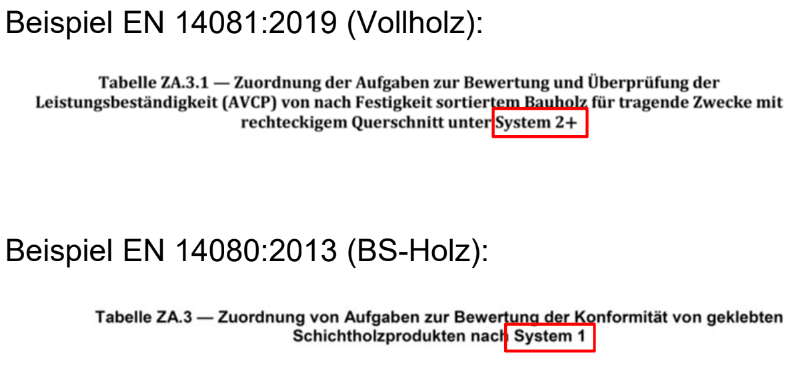
\includegraphics[width=0.9\textwidth]{Grafiken/Einführung/Konformitaetsbesch. Bsp.png}
        \end{minipage}
        \begin{minipage}{0.5\textwidth}
            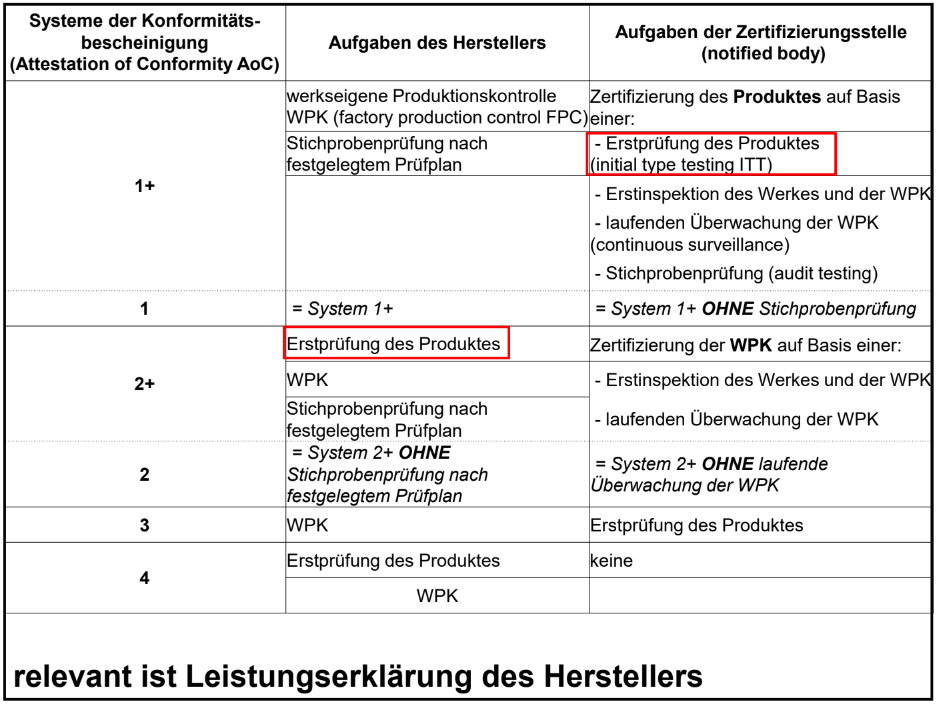
\includegraphics[width=0.9\textwidth]{Grafiken/Einführung/Konformitaetsbesch. Tabelle.png}
        \end{minipage}

    \subsection{Wie sieht es in der Praxis aus?}
        \begin{itemize}
            \item $\rightarrow$ Tabellenwerke von Herstellern
            \item \enquote{Normen ersetzen keine Erfahrung}
            \item Auspassen mit verschiedenen Normen, ETAs und Zulassungen!
                \begin{itemize}
                    \item Beispiel Bestimmung Ausziehtragfähigkeit:\\
                        $\begin{gathered}
                        F_{w, k}=f_{w, k} \cdot \pi \cdot d \cdot L_{\text {ef }} \\
                        f_{a x}=\frac{F_{a x}}{d \cdot L_{e f}} \overset{\text{\Lightning}}{\Longleftrightarrow} F_{a x}=f_{a x} \cdot \pi \cdot d \cdot L_{e f}
                        \end{gathered}$\\
                        Gleiche Variable in verschiedenen Normen, \\
                        aber unterschiedliche Berechnungsweisen und somit statische Bedeutungen
                    \item Festigkeitsklassen Vollholz aus Nadelholz:\\
                        EN 338:2003: $\mathrm{C} 24 \mathrm{f}_{\mathrm{v}, \mathrm{k}}=2,5 \mathrm{MPa}$\\
                        EN 338:2016: $\mathrm{C} 24 \mathrm{f}_{\mathrm{v}, \mathrm{k}}=4,0 \mathrm{MPa}$\\
                        EN 1995-1-1:2010, Abschnitt 6.1.7 Schub: $\tau_d \leq f_{v, d}$\\
                        $\mathrm{f}_{\mathrm{v}, \mathrm{d}}$ wird ermittelt mit $\mathrm{b}_{\mathrm{ef}}=\mathrm{k}_{\mathrm{cr}} \cdot \mathrm{b}$\\
                        und $\mathrm{k}_{\mathrm{cr}}=0,67$ für Vollholz (aufgrund von Schwindrissen)
                \end{itemize}
        \end{itemize}


        
\newpage
\section{CLT – Verbindungen}

Was gibt es generell für Verbindungen:
    \begin{itemize}
        \item Zuganker
        \item Winkel Ableitung Horizontalkraft
        \item CLT-Wandstöße über Sperrholz oder Hartholzbretter verschrauben / über flachen Blattstoß verschrauben
        \item Deckenstoße mit übergreifenden selbstbohrenden Schrauben verbinden 
        \item shear keys aus (Buchen-)Hartholz
    \end{itemize}

Generelle Verbindungsstellen:
    \begin{itemize}
        \item Verbindungen in Bauteilebene
        \item Eckverbindungen
            \begin{itemize}
                \item Von außen verschraubt (Gefahr Hirnholzverschraubung)
                \item Von innen verschraubt
                \item Von innen mit Metallwinkel verschraubt
            \end{itemize}
        \item Wand - Decke Verbindungen\\
            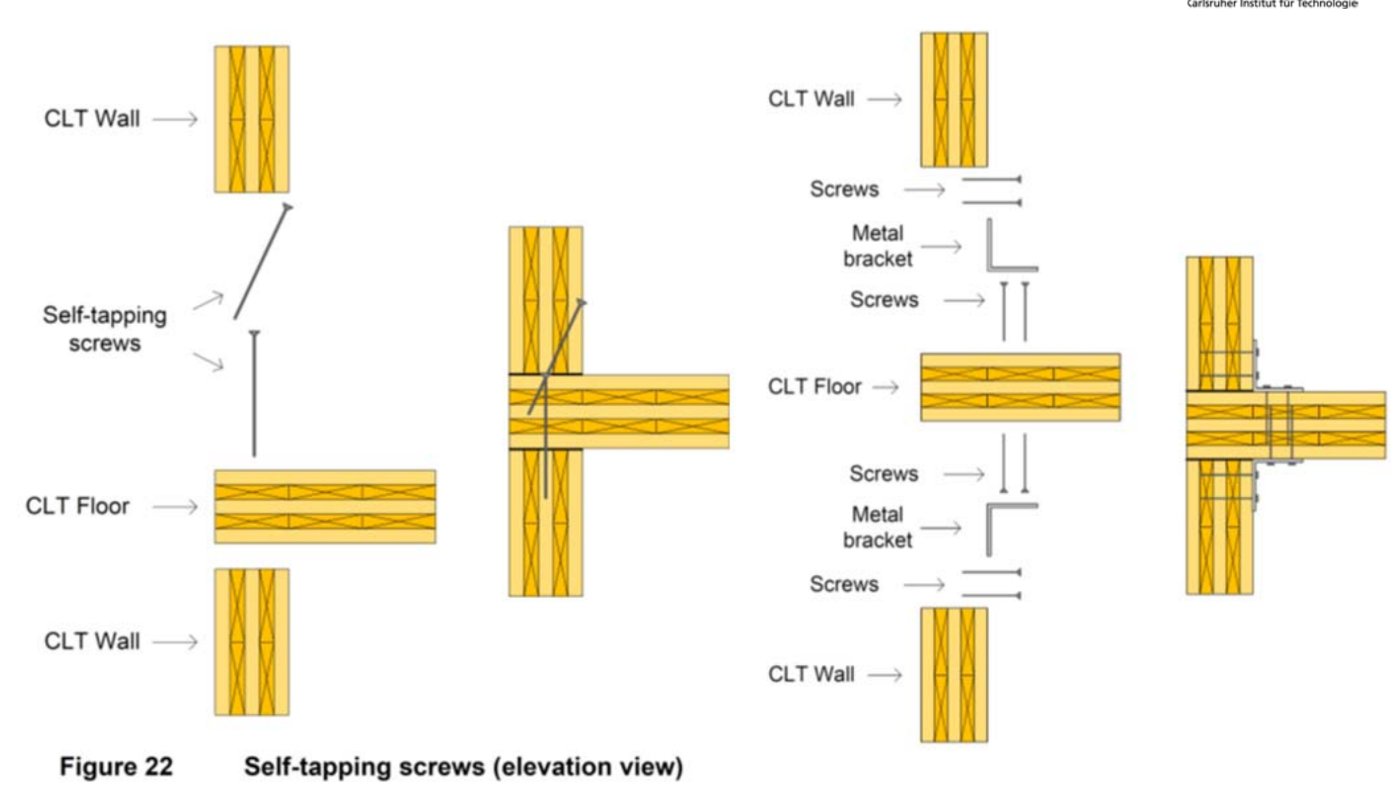
\includegraphics[width=0.45\textwidth]{Grafiken/CLT-Verbindungen/Wand-Decke mit Schrauben.png}
            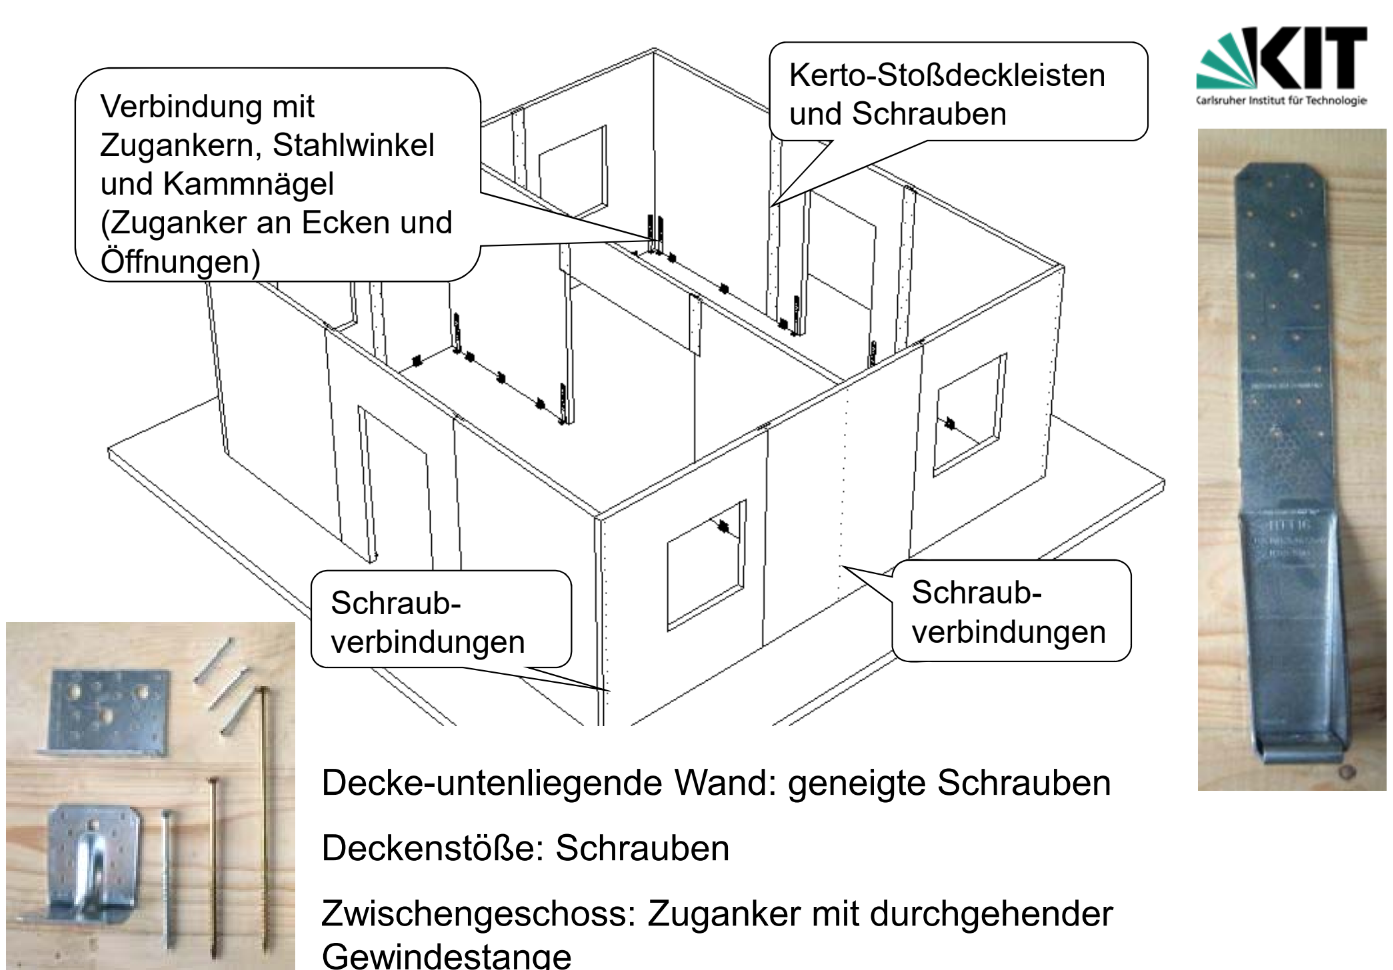
\includegraphics[width=0.45\textwidth]{Grafiken/CLT-Verbindungen/Wand-Decke Uebersicht.png}\\
            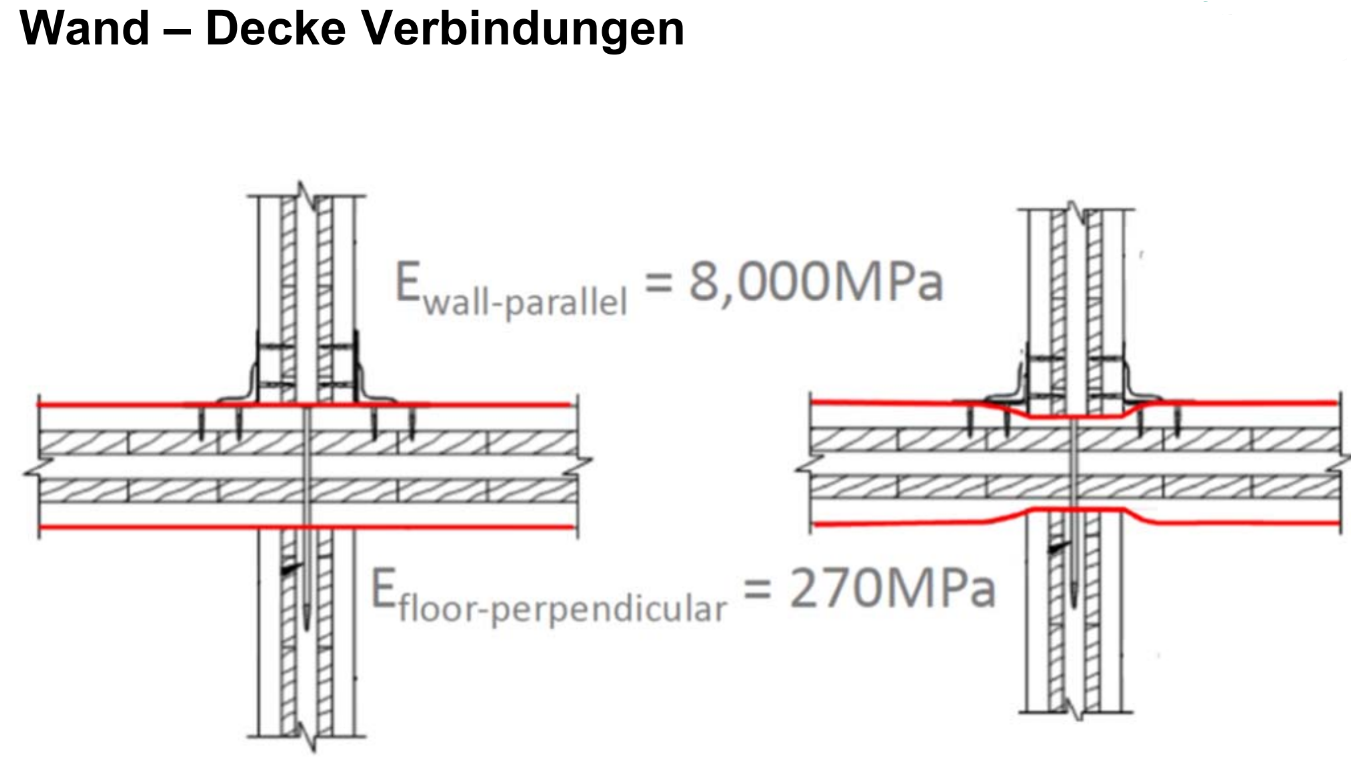
\includegraphics[width=0.45\textwidth]{Grafiken/CLT-Verbindungen/Wand-Decke Pressung.png}
            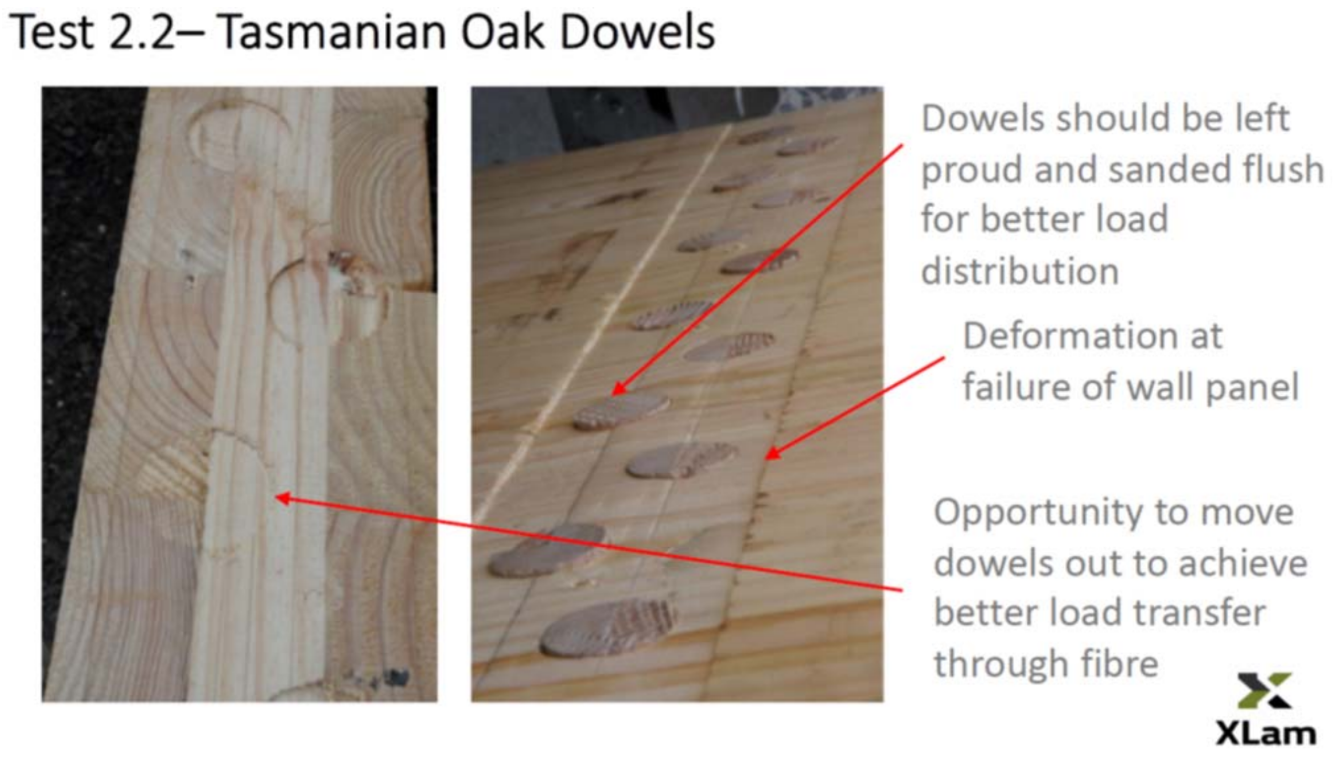
\includegraphics[width=0.45\textwidth]{Grafiken/CLT-Verbindungen/Wand-Decke Dowels.png}\\
            Weitere Dübelarten: Beton, Buchenfurnierschichtholz, eingeschraubte Metallplatten (nicht so gut)\\
            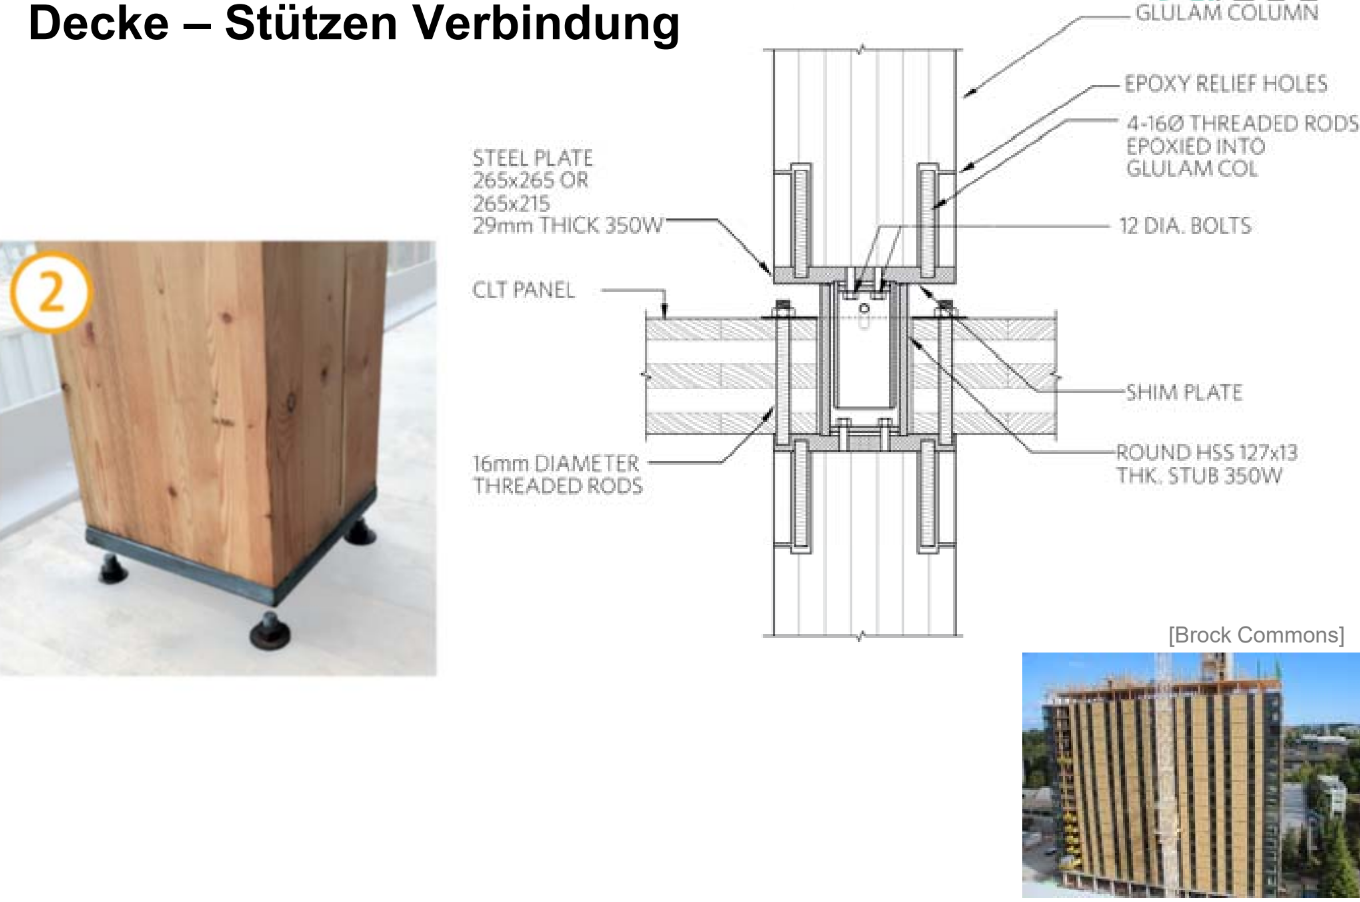
\includegraphics[width=0.45\textwidth]{Grafiken/CLT-Verbindungen/Wand-Decke Pressung Sonerloesung.png}
            
        \item Wand - Dach Verbindungen
            \begin{itemize}
                \item Geneigte Winkel entlang der Dachfußpunkte
            \end{itemize}
        \item Wand - Bodenplatte Verbindungen
            \begin{itemize}
                \item Zuganker
                \item Winkel (in BP verdübelt)
                \item Schlitzbleche auf Fundament aufgebracht und mit selbstbohrenden Stabdübeln mit CLT verbunden
            \end{itemize}
    \end{itemize}

Speziellere Verbindungen:
    \begin{itemize}
        \item CLT auf Zug eingebrachte Bolzen die in Dose zwischen Träger mit Muttern angeschraubt werden (Nachspannbarkeit, Lösbarkeit)\\
        
    \end{itemize}

Besonderheiten CLT:
    \begin{itemize}
        \item Im Vergleich zu Holztafelbau sehr steif $\rightarrow$ Kippt eher als dass es sich verformt, dadurch sehr konzentrierte Last auf Schubverbindungen zwischen Tafelelementen\\
        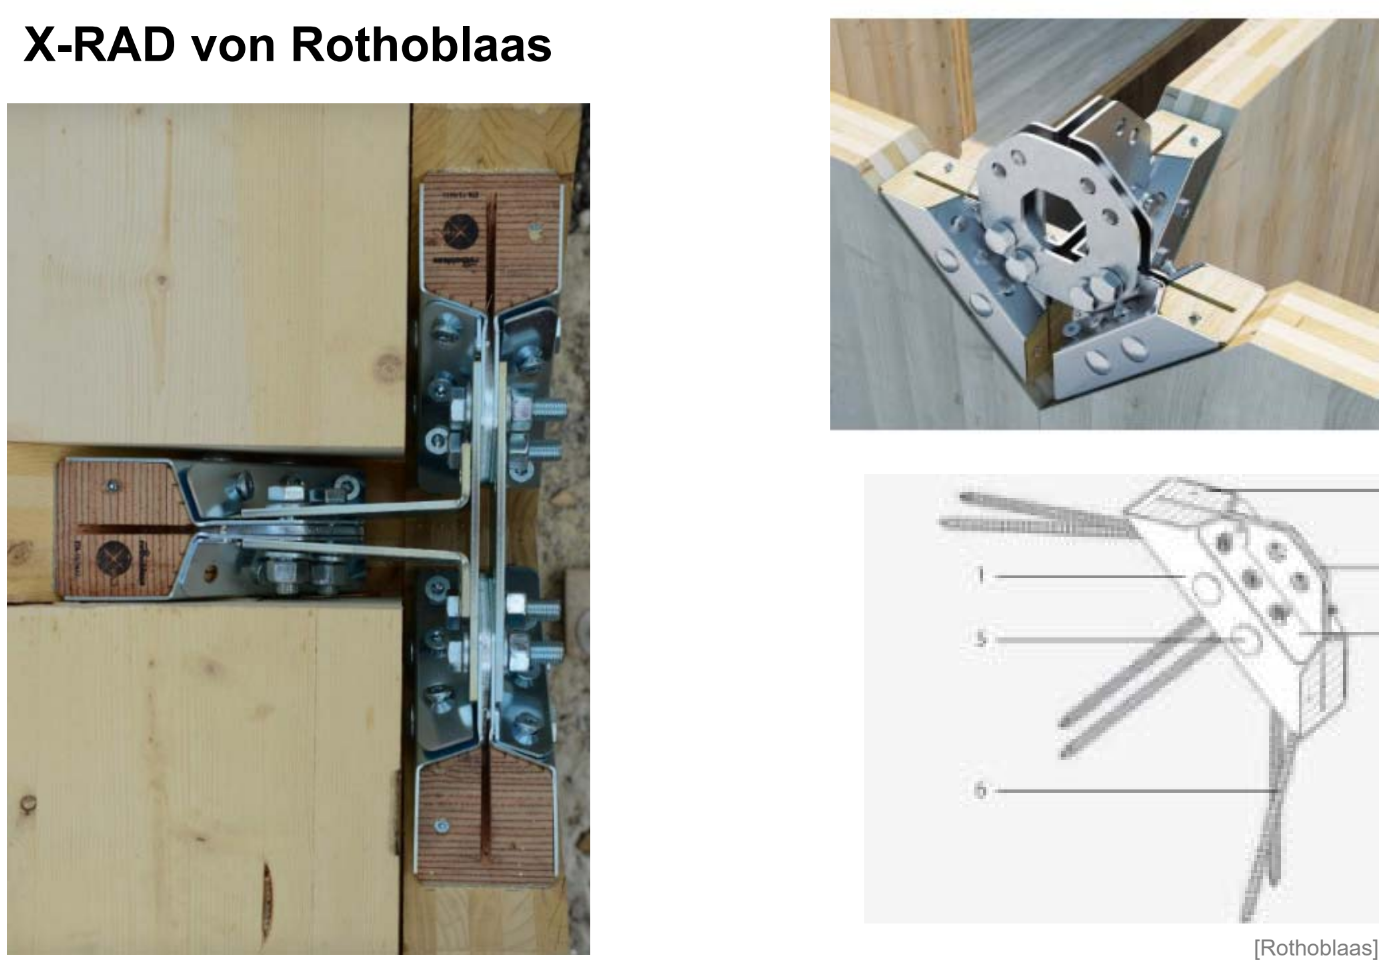
\includegraphics[width=0.45\textwidth]{Grafiken/CLT-Verbindungen/X-RAD Rothoblaas.png}
        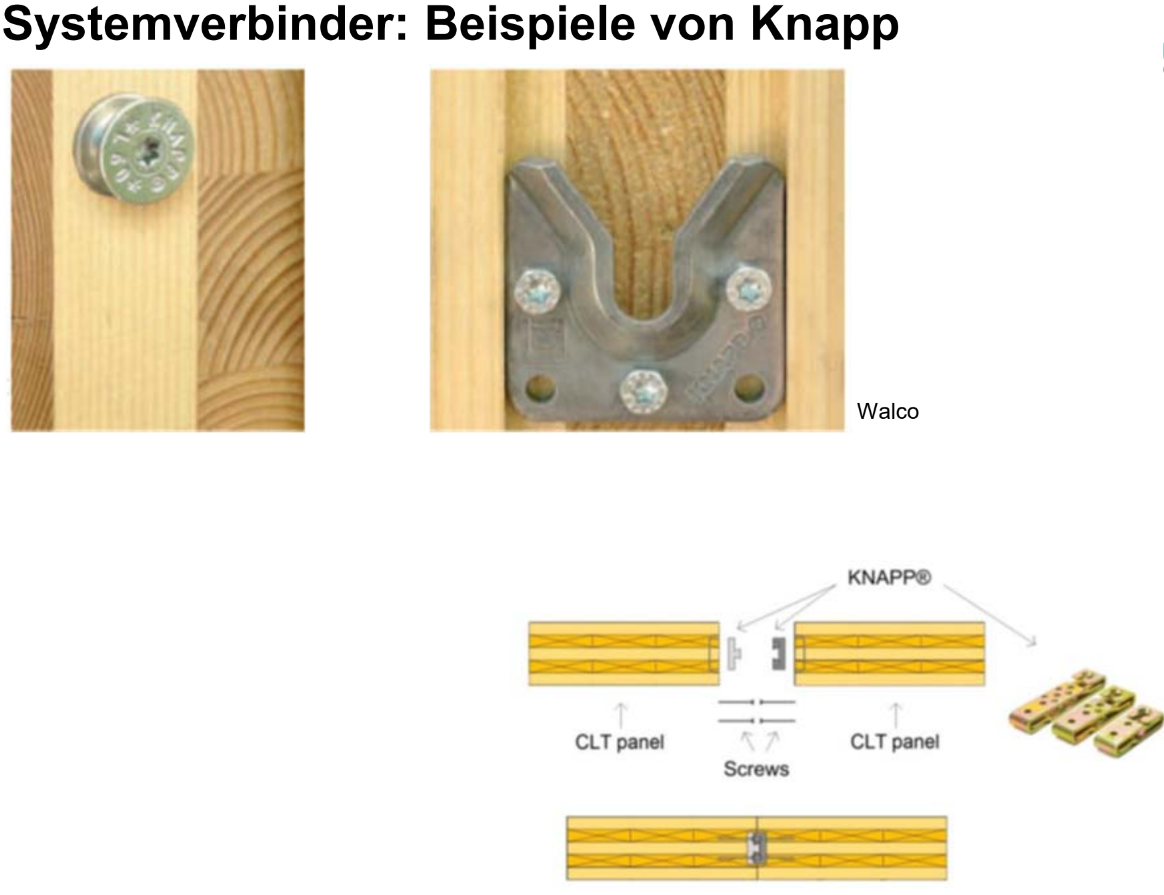
\includegraphics[width=0.45\textwidth]{Grafiken/CLT-Verbindungen/Knapp Systemverbinder.png}\\
        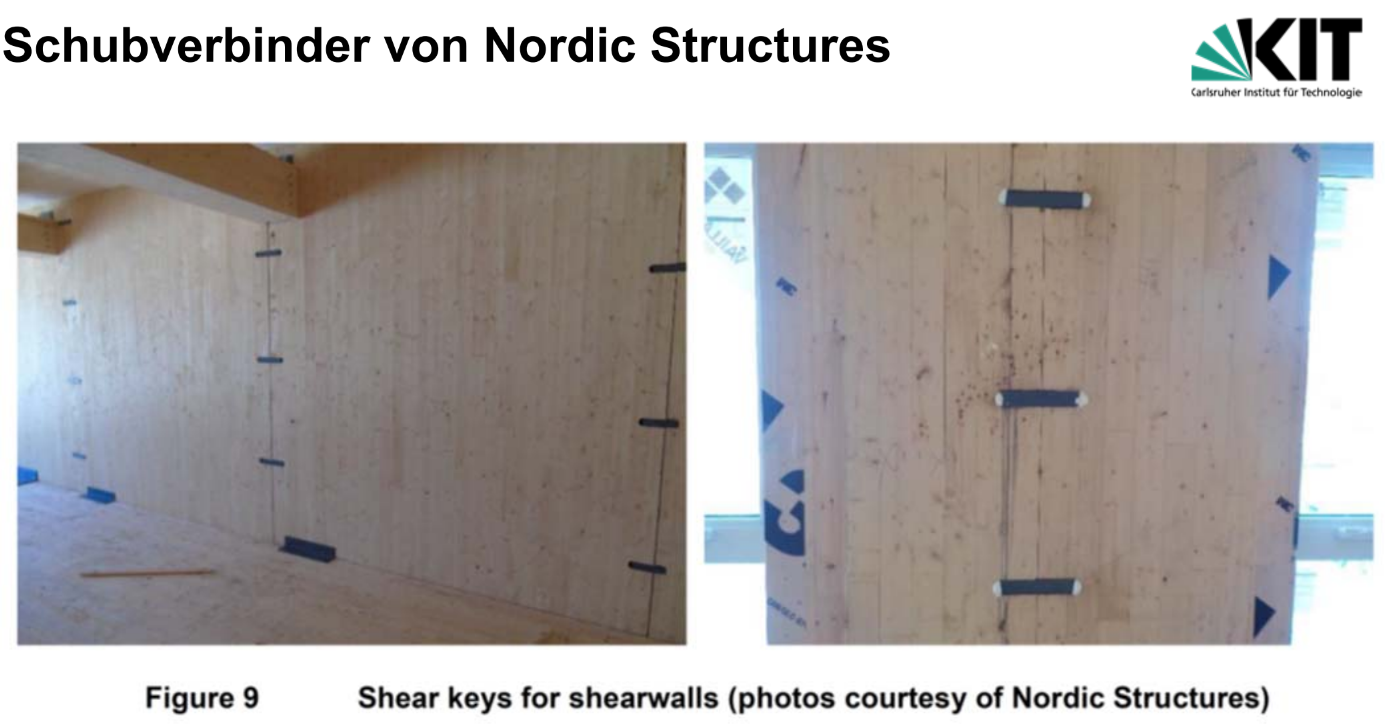
\includegraphics[width=0.45\textwidth]{Grafiken/CLT-Verbindungen/Nordic Structures Schubverbinder.png}
        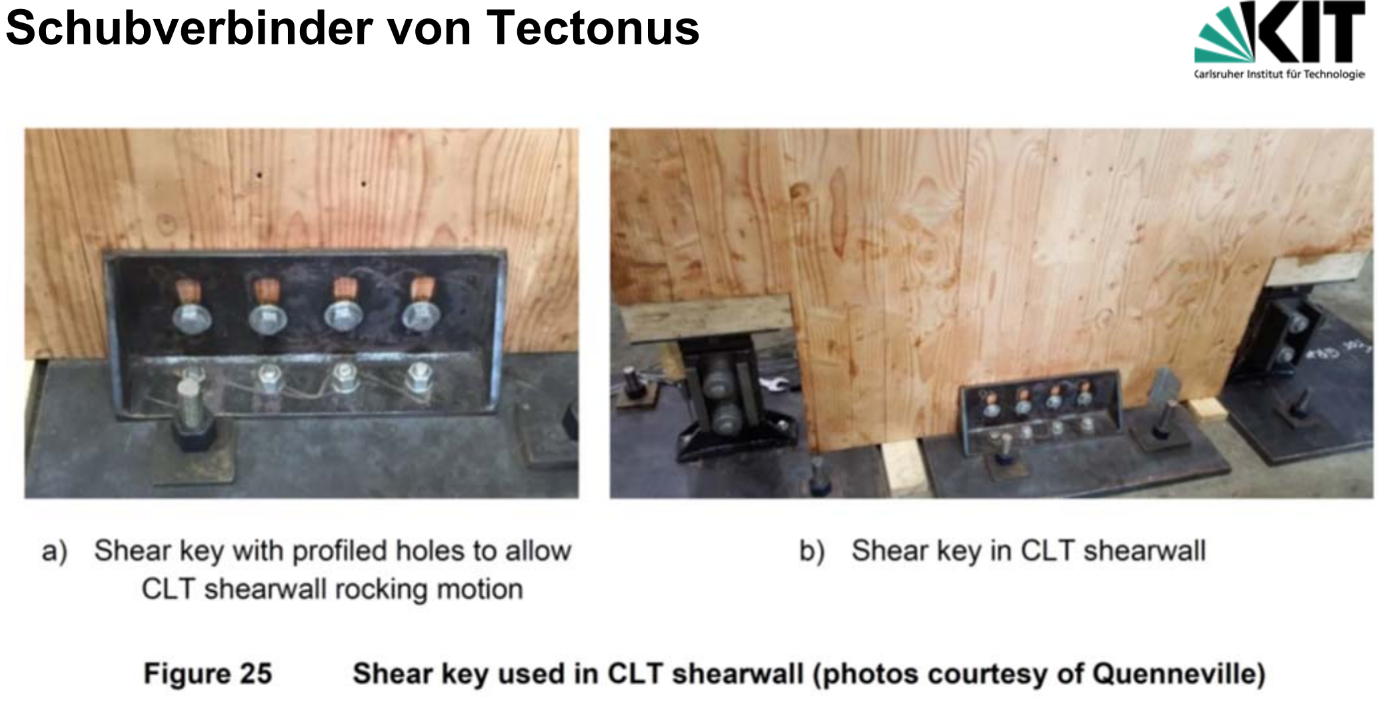
\includegraphics[width=0.45\textwidth]{Grafiken/CLT-Verbindungen/Tectonus Schubverbinder.png}\\
        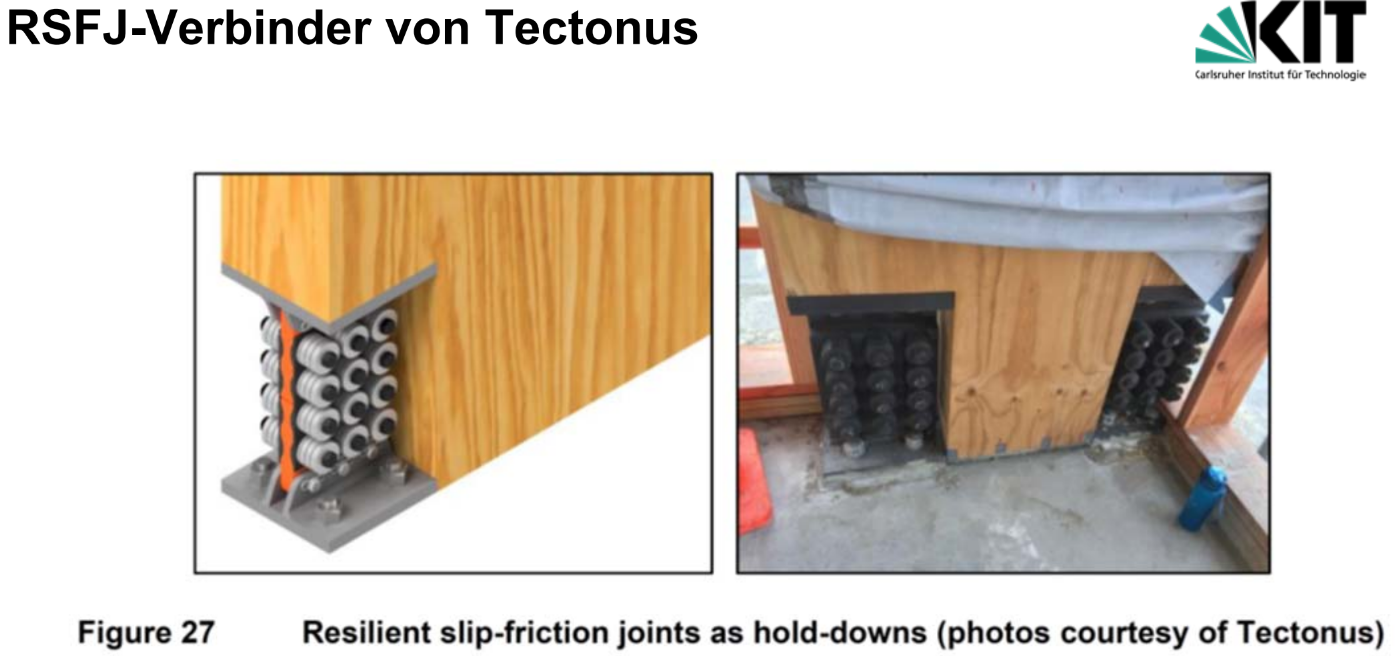
\includegraphics[width=0.45\textwidth]{Grafiken/CLT-Verbindungen/Tectonus RSFJ.png}\\
        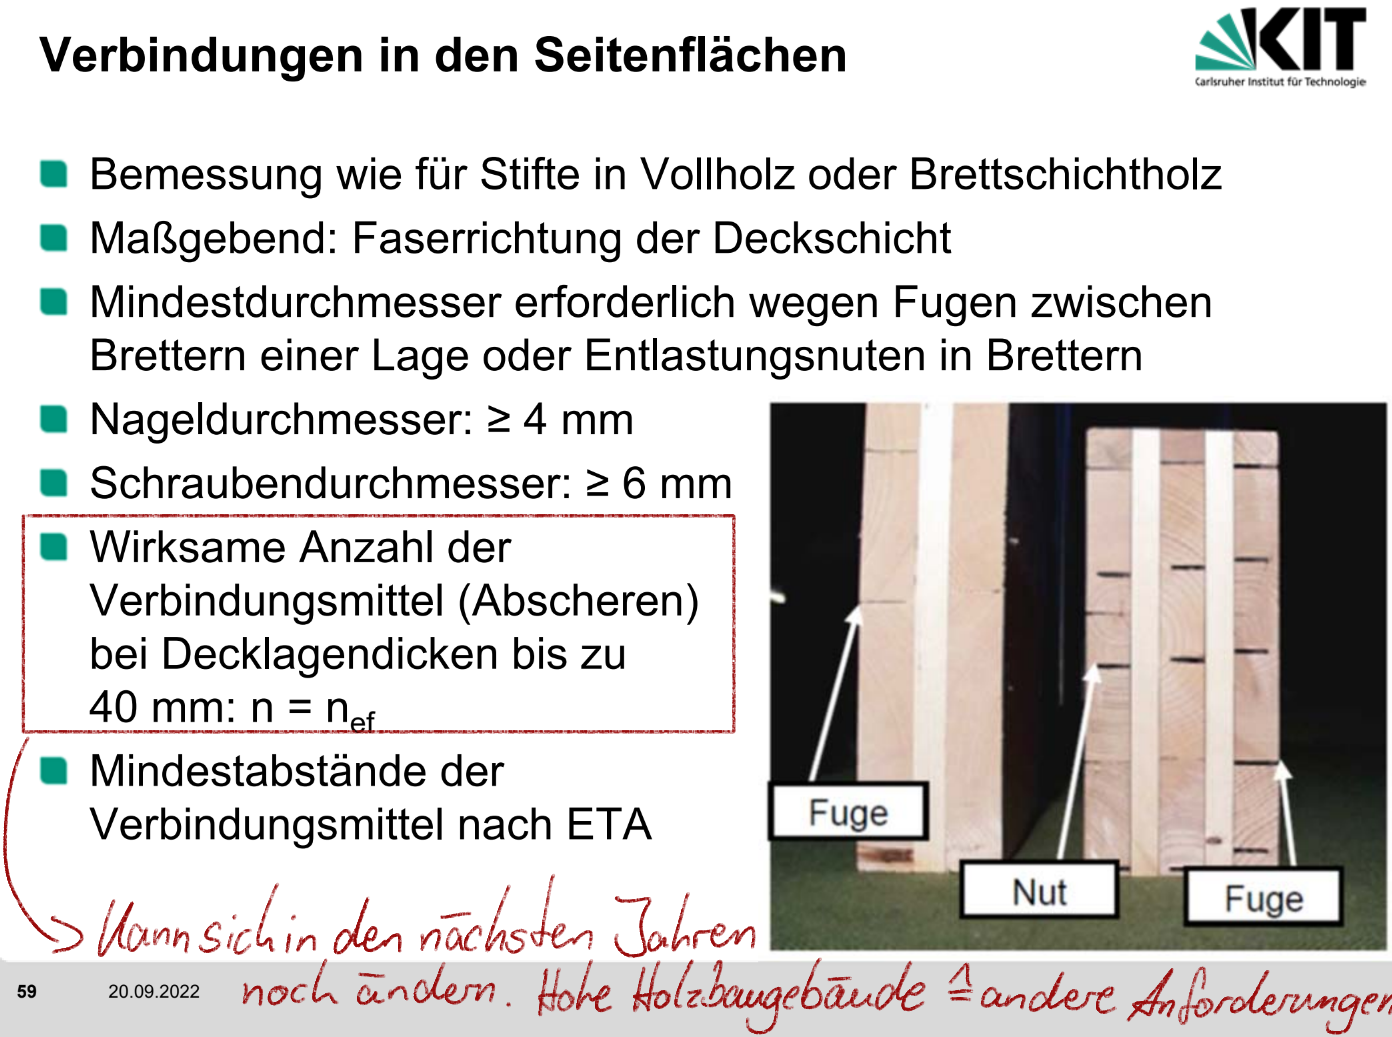
\includegraphics[width=0.45\textwidth]{Grafiken/CLT-Verbindungen/Verbindungen Seitenflächen.png}
        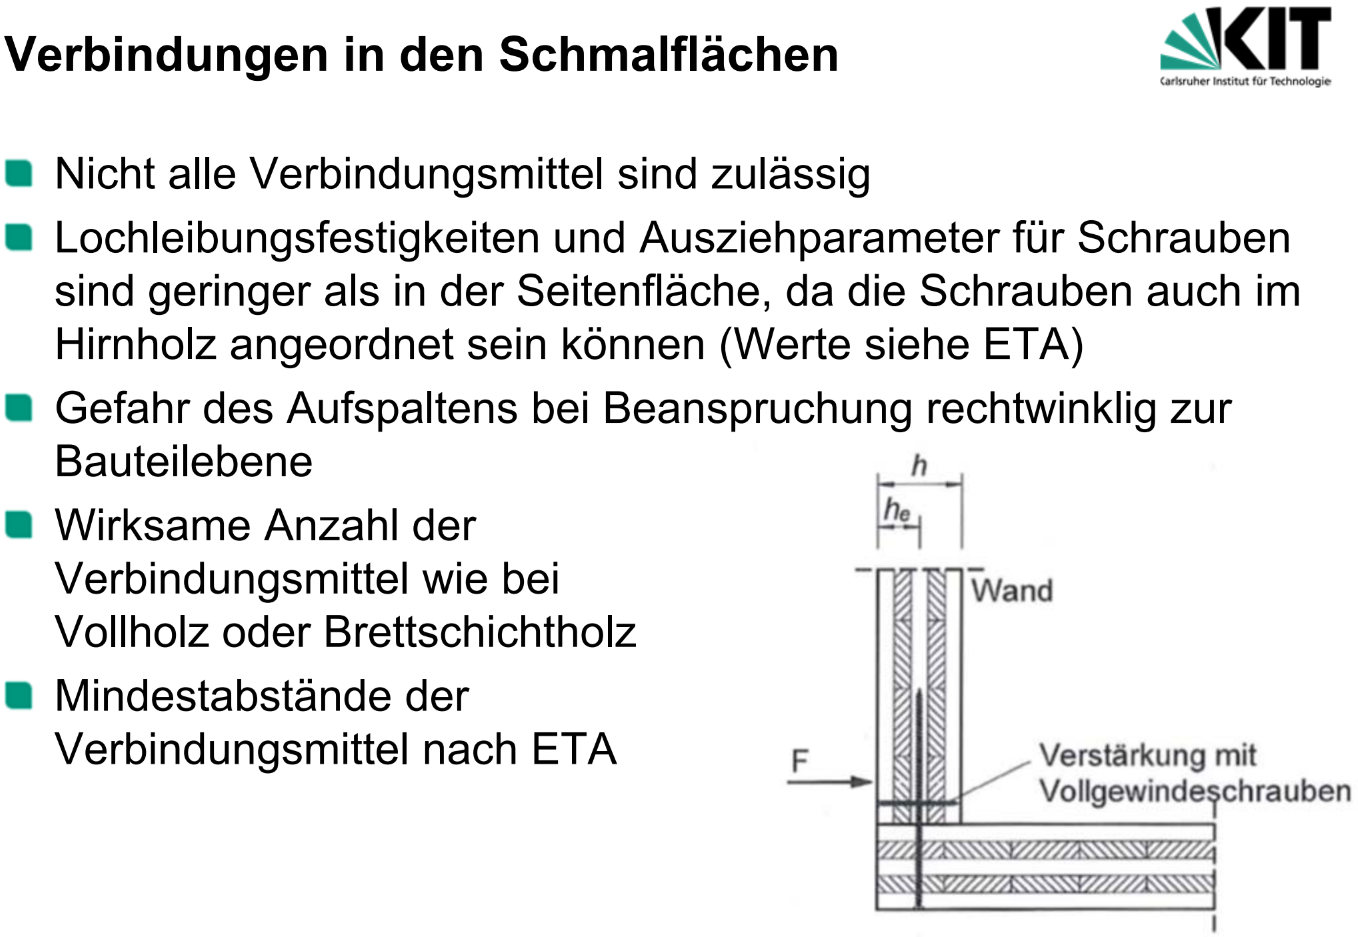
\includegraphics[width=0.45\textwidth]{Grafiken/CLT-Verbindungen/Verbindungen Schmalflaechen.png}\\
        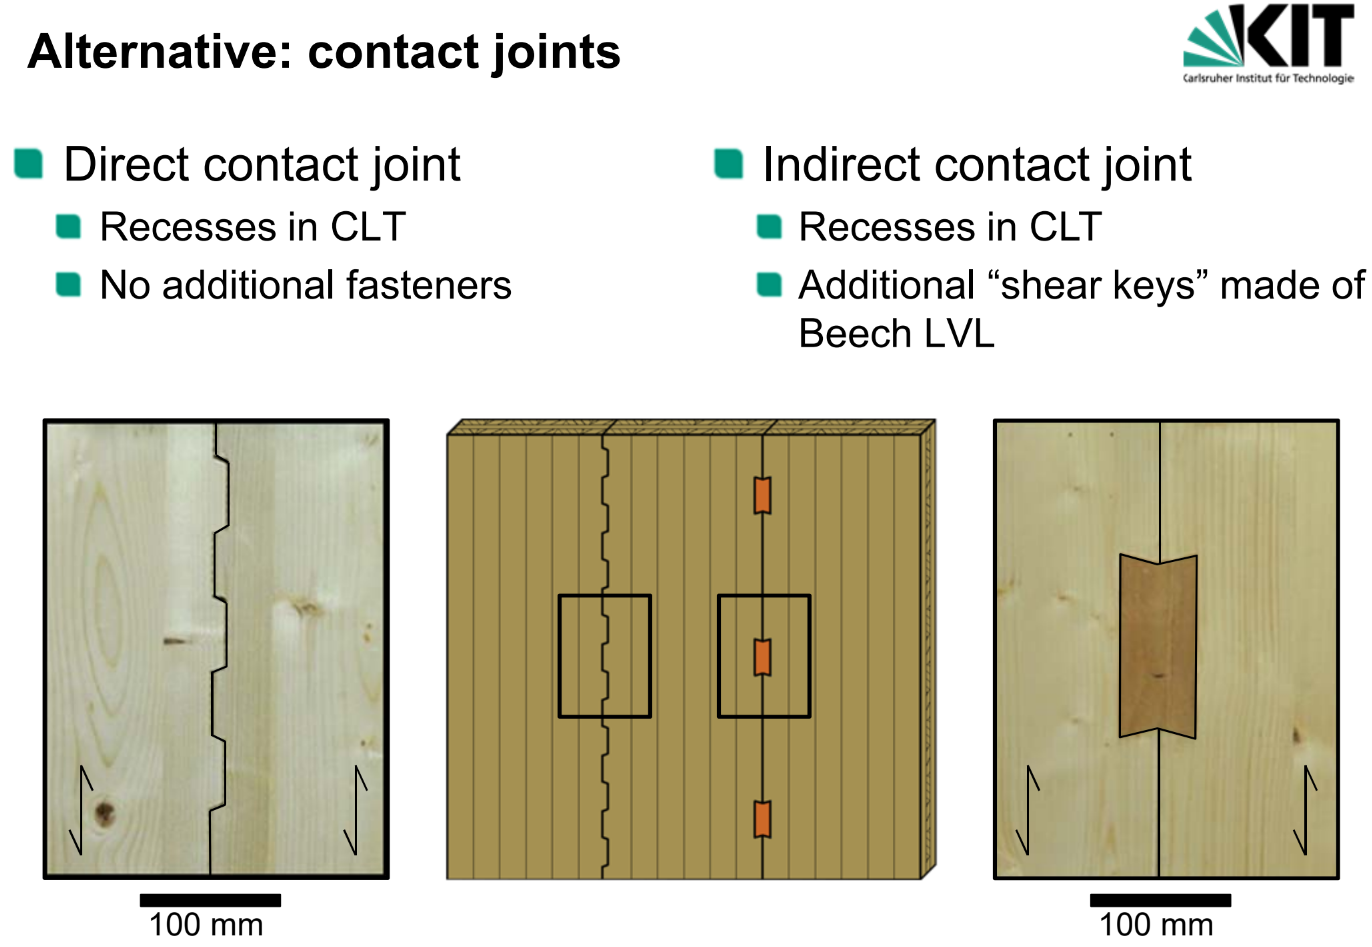
\includegraphics[width=0.45\textwidth]{Grafiken/CLT-Verbindungen/Contact joints.png}\\
        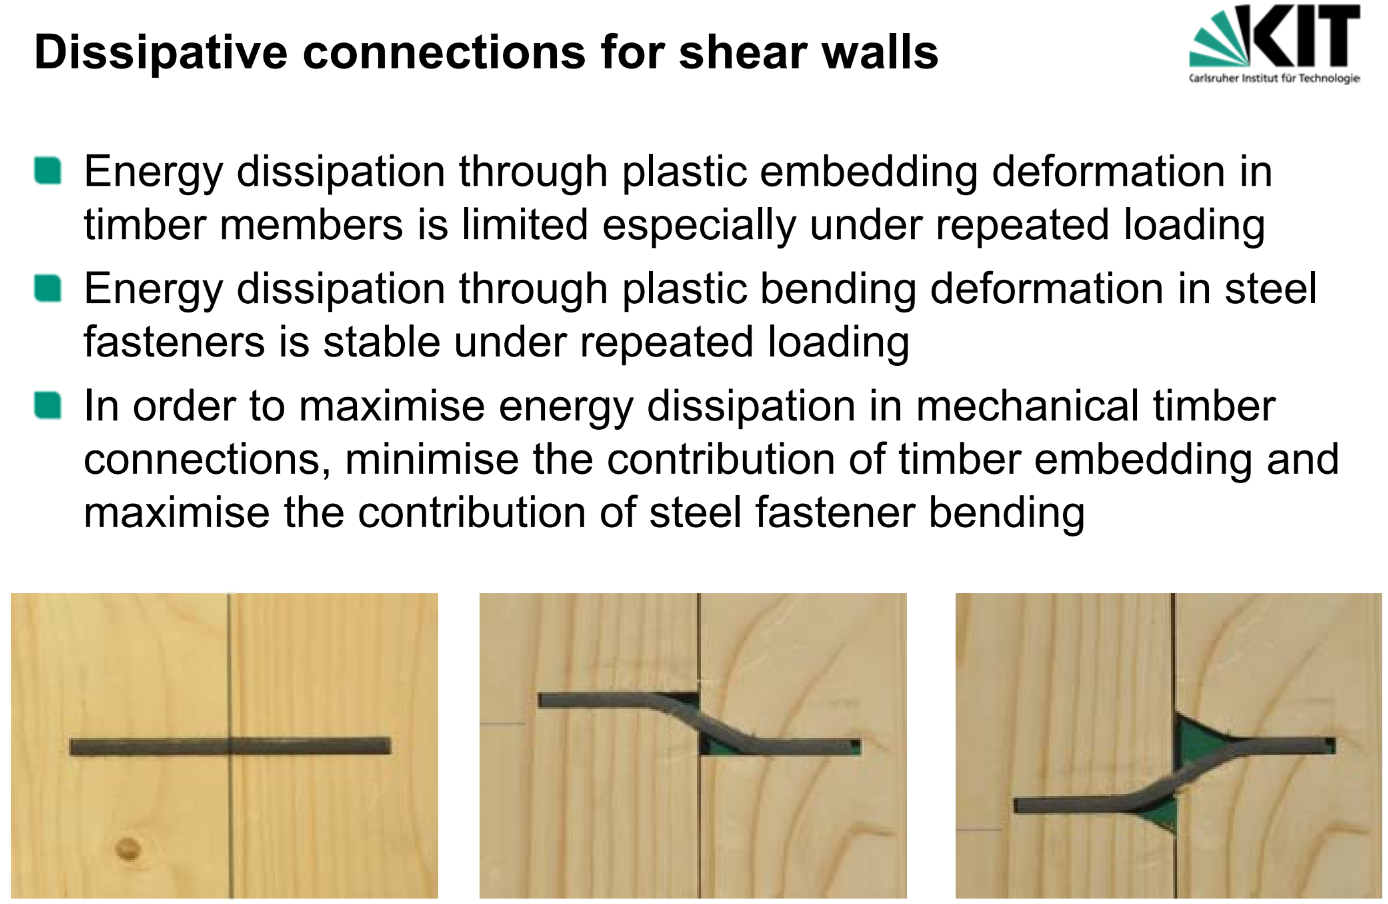
\includegraphics[width=0.45\textwidth]{Grafiken/CLT-Verbindungen/Dissipative joints.png}
        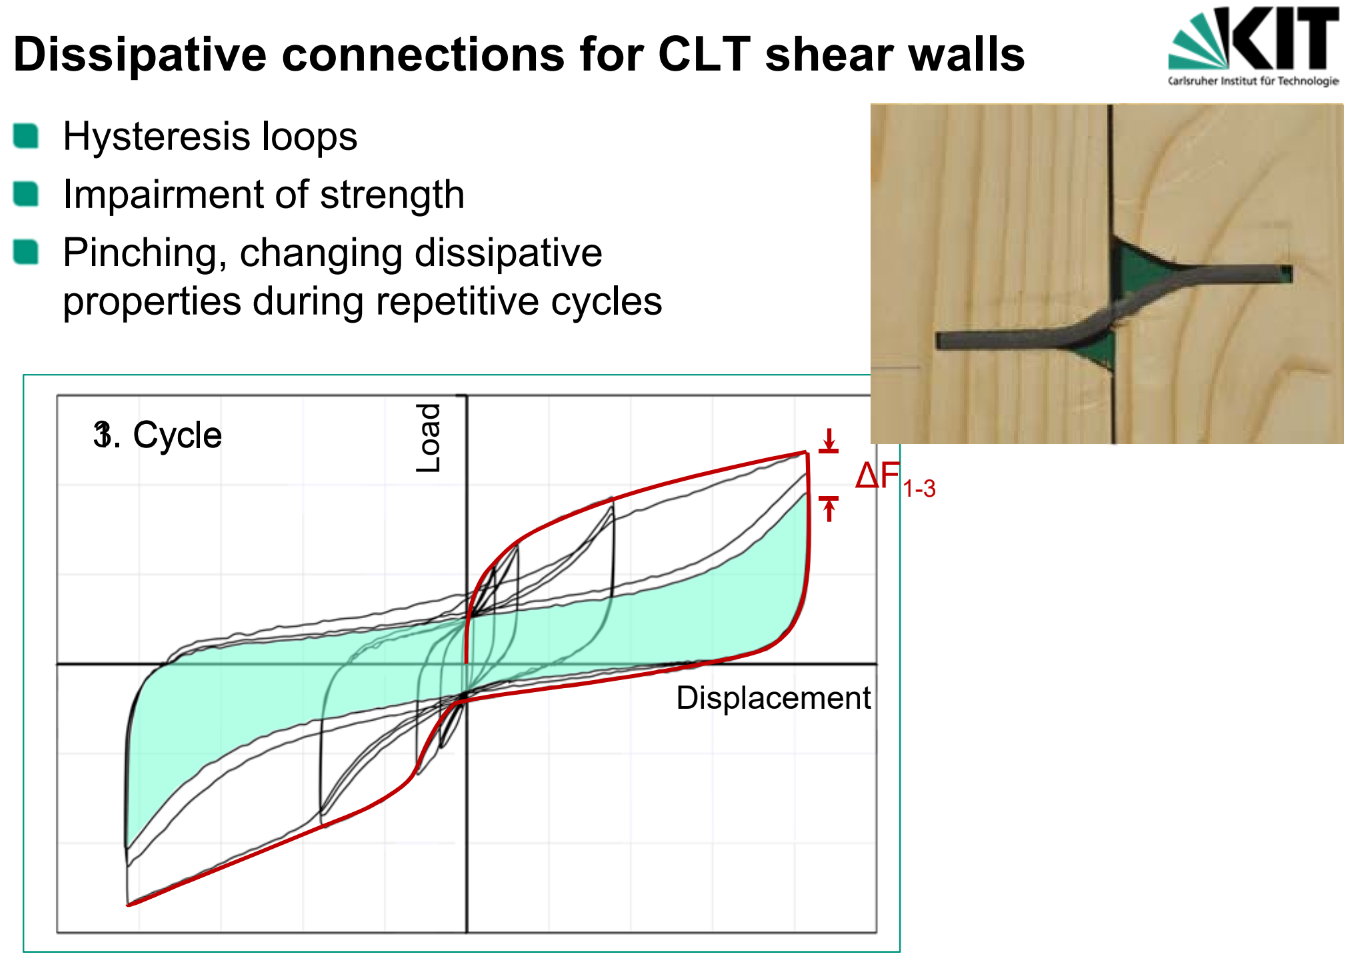
\includegraphics[width=0.45\textwidth]{Grafiken/CLT-Verbindungen/Dissipative joints hysteresis.png}\\
        
    \end{itemize}



\newpage
\section{Laubholz \& Laubholzverbindungen}

    \subsection{Häufige Vertreter}
        Anteile an weltweit verwendeten Holz:
        \begin{itemize}
            \item Fichte (25\%) $\rightarrow$ NH
            \item Kiefer (23\%) $\rightarrow$ NH
            \item Buche (15\%) $\rightarrow$ LH
            \item Eiche (10\%) $\rightarrow$ LH
            \item Weitere LH: Esche, Birke, Erle, Ahorn, Pappel, Hainbuche
            \item Tendenz Laubholznutzung steigend (Fichtenwachstum rückgängig)
        \end{itemize}

    \subsection{Generelles}
        \begin{itemize}
            \item Historische Nutzung: Bauholz, Möbelbau, Schiffbau, Brennholz, Holzkohle, Teller/Besteck und Kunst (schwer zu verarbeiten, da sehr hart)
            \item Ötzi Nutzung Hartholzvarianten zu jeweiligen Stärken
            \item Aktuelle Nutzung:
                \begin{itemize}
                    \item In Zahlen:\vspace*{3mm} \\
                            \resizebox{0.9\textwidth}{!}{%
                            \begin{tabular}{|c|c|c|c|c|c|}
                            \hline
                            {[}Mio.Fm{]} & Entnahme & Sägeindustrie & Holzwerkstoffindustrie & Holzstoff/Zellstoff & Furnier-/Sperrholz \\ \hline
                            Energetische Nutzung: & 13,9 (70\%) &  &  &  &  \\ \hline
                            Stoffliche Nutzung: & 5,9 (30\%): & 2,6 (44\%) & 2,4 (40\%) & 0,7 (12\%) & 0,2 (4\%) \\ \hline
                            Gesamt: & 19,8 (100\%) & \multicolumn{1}{l|}{} & \multicolumn{1}{l|}{} & \multicolumn{1}{l|}{} & \multicolumn{1}{l|}{} \\ \hline
                            \end{tabular} } \vspace{1mm}
                    \item Schlussfolgerung:\\
                        Laubholz kann Nadelholz nicht vollständig substituieren: mangelnde Verfügbarkeit und technologische Schwierigkeiten (Verarbeitung \& Verklebung z.T. schwierig, wesentlich kürzere Standzeiten von Bearbeitungswerkzeugen, erhöhte Quellund Schwindmaße,..)\\
                        Daraus folgende Frage:
                            Wie kann Laubholz maßgeschneidert eingesetzt werden?
                                \begin{itemize}
                                    \item Höhere Rohdichte als Nadelholz $\rightarrow$ höhere Festigkeit
                                    \item Höhere Dauerhaftigkeit einiger LH-Arten:\\
                                        Robinie hat Dauerhaftigkeitsklasse 1-2 von 5 gegen Pilze\\
                                        (1 - \enquote{sehr dauerhaft} bis 5- \enquote{nicht dauerhaft} )
                                \end{itemize}
                \end{itemize}
        \end{itemize}

    \subsection{Relevante Holzprodukte}
        \begin{itemize}
            \item Vollholz
            \item Brettschichtholz (BS-Holz/BSH/GLT)
            \item Brettsperrholz (BSP/CLT)
            \item Furnierschichtholz (FSH)
            \item Furniersperrholz
        \end{itemize}
    \subsection{Eigenschaften und Bemessung}
        \begin{itemize}
            \item Unterschiede Nadelholz - Laubholz:
                \begin{itemize}
                    \item Nadelholz ist evolutionär weniger weit entwickelt als Laubholz
                    \item Laubholz ist ausdifferenzierter in seinem anatomischen Aufbau (Nadelholz hat nur sog. \enquote{Tracheiden} als Zelltypen)
                    \item Nadelholz ist i. a. \enquote{langfasrig} und Laubholz \enquote{kurzfasrig}
                    \item Klebeigenschaften sind z.T. anders
                    \item Bearbeitung von LH ist oft schwieriger
                    \item Laubholzprodukte i. a. teurer als Nadelholzprodukte
                \end{itemize}
             \newpage   
            \item Links: Aufbau BaumQS Rechts: Faser-/Zellstruktur\\
                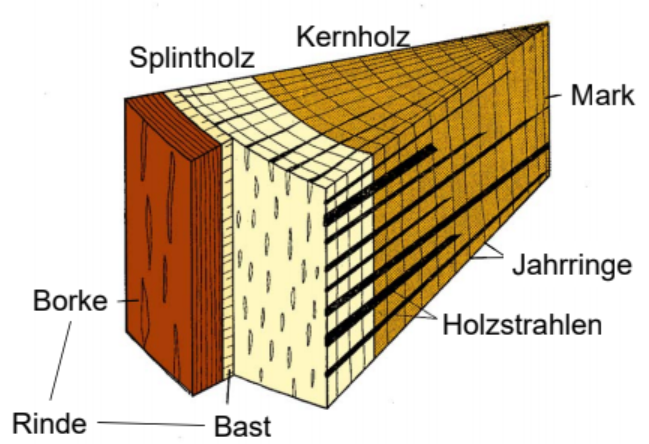
\includegraphics[width=0.4\textwidth]{Grafiken/Laubholz/BaumQS.png}
                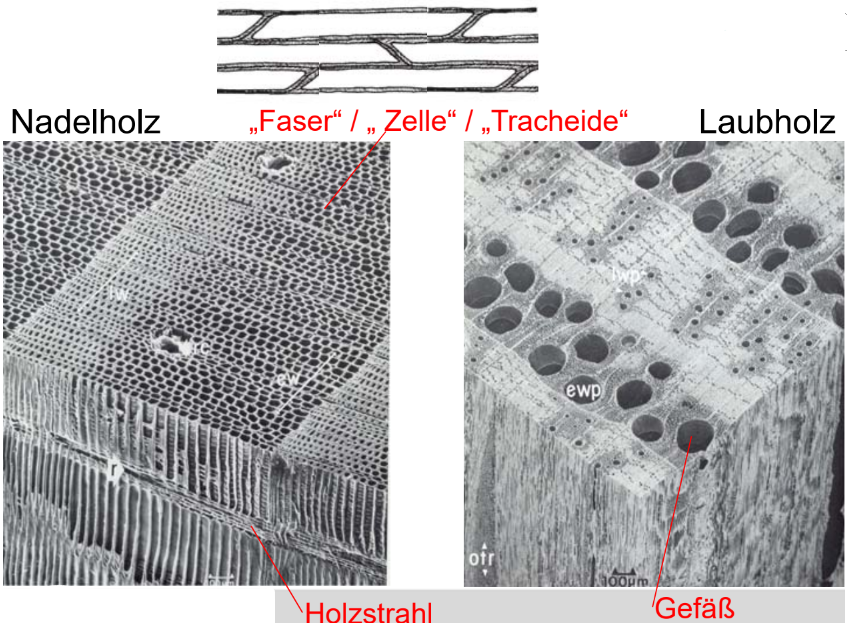
\includegraphics[width=0.4\textwidth]{Grafiken/Laubholz/Zellstruktur.png}\\
            \item Laubholzanatomie:
                \begin{itemize}
                    \item sehr vielfältig
                    \item Viele verschiedene Zelltypen:
                        \begin{itemize}
                            \item  verschiedene Tracheiden mit unterschiedlichen Funktionen:
                            z. B. \enquote{Libriformfaser} zur Festigung und
                            \enquote{Fasertracheide} zur Wasserleitung
                            \item  Gefäße zur Wasserleitung, je nach LH-Art unterschiedlich
                            \item  Parenchym zur Speicherung
                        \end{itemize}
                    \item Umwandung von Splint zu Kern ist holzartspezifisch
                        \begin{itemize}
                            \item  Einlagerung von Inhaltsstoffen mit versch. Funktionen: Farbstoffe, Gerbstoffe, Fette, Harze, Phenole, Terpene
                            \item versch. Mechanismen zum Zellabschluss, z.B. Verthyllung
                        \end{itemize}
                \end{itemize}
            \item Rohdichte und Holzfeuchte
                \begin{itemize}
                    \item LH-Arten haben wegen unterschiedlichen anatomischen Aufbaus unterschiedliche Rohdichten:\\
                    Balsaholz ca. $100 \mathrm{~kg} / \mathrm{m}^3 \Longleftrightarrow$ Pockholz ca. $1200 \mathrm{~kg} / \mathrm{m}^3$
                    \item Zusätzlich bestimmen noch weitere Faktoren die Rohdichten, z.B. die Wuchsbedingungen
                    \item Holz ist hygroskopisch und seine Eigenschaften sind bis zum Fasersättigungsbereich feuchteabhängig
                    \item Holzfeuchteänderungen unterhalb des Fasersättigungsbereichs führen zu Schwind- und Quellverformungen
                    \item Schwindverformungen tangential sind am größten
                \end{itemize}
                    $\Rightarrow$ Betrachtung auf Holzartebene bei LH wichtiger als bei NH
            \item Eigenschaften und Verwendung:
                \begin{itemize}
                    \item Hainbuche/Weißbuche:
                        \begin{itemize}
                            \item Hohes Schwindmaß, nicht relevant für Bauwesen
                            \item Verwendung: Werkzeugbau, Klavierbau
                        \end{itemize}
                    \item Pappel:
                        \begin{itemize}
                            \item Nicht dauerhaft
                            \item Verwendung: Papierindustrie
                            \item Bauwesen: Holzwerkstoffplatten, BS-Holz
                        \end{itemize}
                    \item Bergahorn:
                        \begin{itemize}
                            \item Nicht dauerhaft, nicht relevant für Bauwesen
                            \item Verwendung: Möbel, Parkett
                        \end{itemize}
                    \item Schwarzerle:
                        \begin{itemize}
                            \item Nur unter Wasser dauerhaft
                            \item Nicht relevant für Bauwesen
                        \end{itemize}
                    \item Robinie:
                        \begin{itemize}
                            \item Sehr dauerhaftes Holz
                            \item Verwendung: Spielplätze
                            \item Bauwesen: Rundholz oder BS-Holz
                        \end{itemize}
                    \item Esche:
                        \begin{itemize}
                            \item Nicht dauerhaft
                            \item Hartes und elastisches Holz
                            \item Verwendung: Wekzeug, Möbel Parkett, Thermoholz
                            \item Bauwesen: BS-Holz, BSP, FSH
                        \end{itemize}
                    \item Gemeine Birke:
                        \begin{itemize}
                            \item Nicht dauerhaft
                            \item Stört Abbinden von Zement
                            \item Verwendung: Sperrholz
                            \item Bauwesen: Sperrholz, BS-Holz, BSP, FSH
                        \end{itemize}
                    \item Edelkastanie:
                        \begin{itemize}
                            \item Dauerhaft
                            \item Bauwesen: BS-Holz
                        \end{itemize}
                    \item Stieleiche:
                        \begin{itemize}
                            \item Wenig bis Dauerhaft
                            \item Reich an Gerbsäure
                            \item Verwendung: Bauwesen, Möbel, Parkett, Innenausbau
                            \item Bauwesen: BS-Holz, BSP
                        \end{itemize}
                    \item Rotbuche:
                        \begin{itemize}
                            \item Nicht dauerhaft
                            \item Verwendung: Sperrholz, Möbelbau, Werkzeugindustrie
                            \item Bauwesen: Sperrholz, BS-Holz, BSP, FSH
                        \end{itemize}
                \end{itemize}
                Übersicht: \vspace*{3mm}\\
                    $\begin{array}{|c|c|c|c|c|}
                        \hline \text { Holzart } & \begin{array}{c}
                        \text { Rohdichte in } k g / m^3 \\
                        \text { (bei ca. 12\% ~ )} 
                        \end{array} & \begin{array}{c}
                        \text { Schwindmaß } \\
                        \text { radial }
                        \end{array} & \begin{array}{c}
                        \text { Schwindmaß } \\
                        \text { tangential }
                        \end{array} & \text { Dauerhaft } \\
                        \hline \text { Fichte } & 330 \ldots 470 \ldots 680 & 0,17 \% & 0,32 \% & \text { nein } \\
                        \hline \text { Pappel } & 400 \ldots 450 \ldots 560 & 0,16 \% & 0,28 \% & \text { nein } \\
                        \hline \text { Robinie } & 720 \ldots 790 \ldots 950 & 0,23 \% & 0,35 \% & \text { ja } \\
                        \hline \text { Esche } & 450 \ldots 690 \ldots 860 & 0,19 \% & 0,33 \% & \text { nein } \\
                        \hline \text { Birke } & 510 \ldots 650 \ldots 830 & 0,21 \% & 0,29 \% & \text { nein } \\
                        \hline \text { Eßkastanie } & 590 \ldots 620 \ldots 660 & 0,15 \% & 0,24 \% & \text { ja } \\
                        \hline \text { Eiche } & 430 \ldots 690 \ldots 960 & 0,19 \% & 0,32 \% & \text { ja - jein } \\
                        \hline \text { Buche } & 540 \ldots 720 \ldots 910 & 0,21 \% & 0,41 \% & \text { nein } \\
                        \hline
                    \end{array}$
                \vspace*{3mm}
                \item Bemessung Laubholz:
                    \begin{itemize}
                        \item Baubuche: 
                            \begin{itemize}
                                \item Baubuche = Buchenfurnierschichtholz
                                \item NKL 3 auf gar keinen Fall, sehr feuchtempfindlich, geht auch nicht mehr ganz zurück
                                \item Homogenisierter QS
                            \end{itemize}
                                \item Problematik mit richtungsabhängiger, komplizierter Bemessung durch Schichtenaufbau
                                \item Brettsperrholz vs Brettstapelholz \\
                                    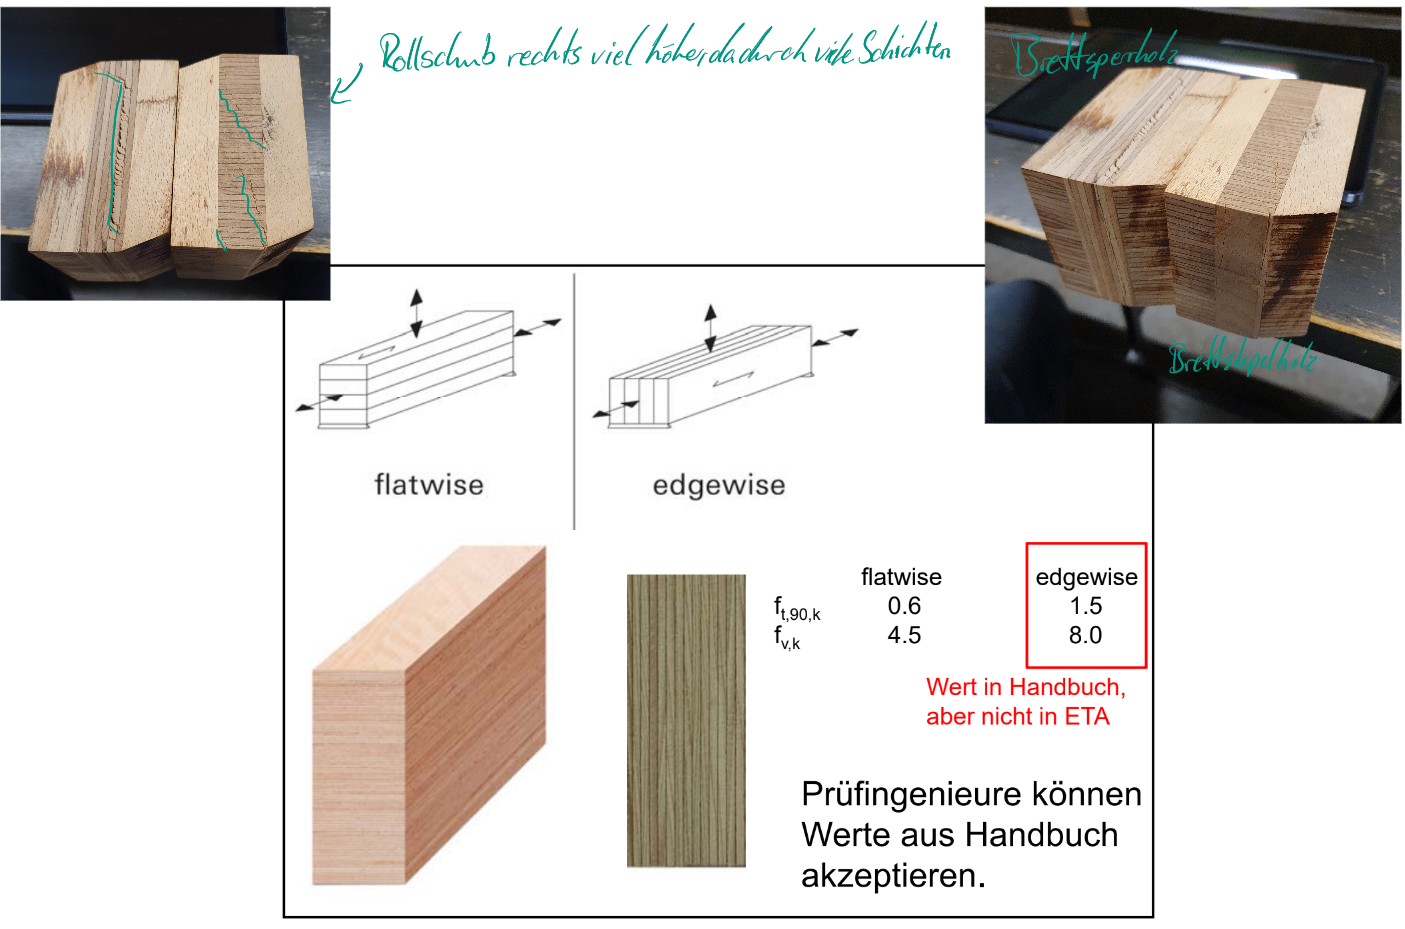
\includegraphics[width=0.4\textwidth]{Grafiken/Laubholz/Baubuche Brettsperr-Brettstapel.png}
                        \item Ausnutzen hoher Festigkeiten schwierig, da andere Versagen vorher eintreten. Lösungen:
                            \begin{itemize}
                                \item Aufgelöste Tragwerke (Fachwerk)
                                \item Hybride Produkte (kombiniertes BS-Holz, Furnier in Zug-/Druckzone, homogener Holzwerkstoff)
                                \item Lokale Verstärkungen
                                \item Ausnutzung der hohen Druckfestigkeiten
                            \end{itemize}
                    \end{itemize}
        \end{itemize}



\newpage
\section{Holzfeuchte}
    
    \subsection{Ziele des Themenbereichs}
        \begin{itemize}
            \item Holzfeuchte und die Reaktion von Holzbauteilen auf Holzfeuchteänderungen
            \item Klimatische Umgebungsbedingungen als Resultat der Gebäudenutzung und der Einfluss unterschiedlicher Umgebungsbedingungen auf die Holzfeuchte von Holzbauteilen
            \item Effekte von Holzfeuchteänderungen auf tragende Holzbauteile und ihre Lastabtragungsmechanismen
            \item Einfluss von Verstärkungselementen auf das Verhalten von Holzbauteilen bei Schwindbeanspruchung und Maßnahmen zur Reduzierung dieser Effekte
        \end{itemize}
    \subsection{Wiederholung}
        \begin{itemize}
            \item Hygroskopisches Material: Materialien die sich Feuchtigkeit anpassen
            \item Fasersättigungspunkt $\rightarrow$ Holzfasern komplett gefüllt $\rightarrow$ Hohlräume füllen sich mit Wasser
            \item Gleichgewichtsfeuchte $\rightarrow$ Passt sich relativer Luftfeuchtigkeit an \\
                    $\rightarrow$ nicht 1:1 (z.B. Luft $60 \% \leftrightarrow$ Holz 12\%)
            \item Holzfeuchtebestimmung $\rightarrow$ elektrischer Widerstand, Darrtrochnngsmethode
            \item Holzfeuchte - Mechanische Eigenschaften
            \item Nutzungsklassen
            \item Schwindmaße: 1\% Feuchteänderung $\rightarrow$ $\frac{1}{4}$\% Längenänderung
        \end{itemize}
    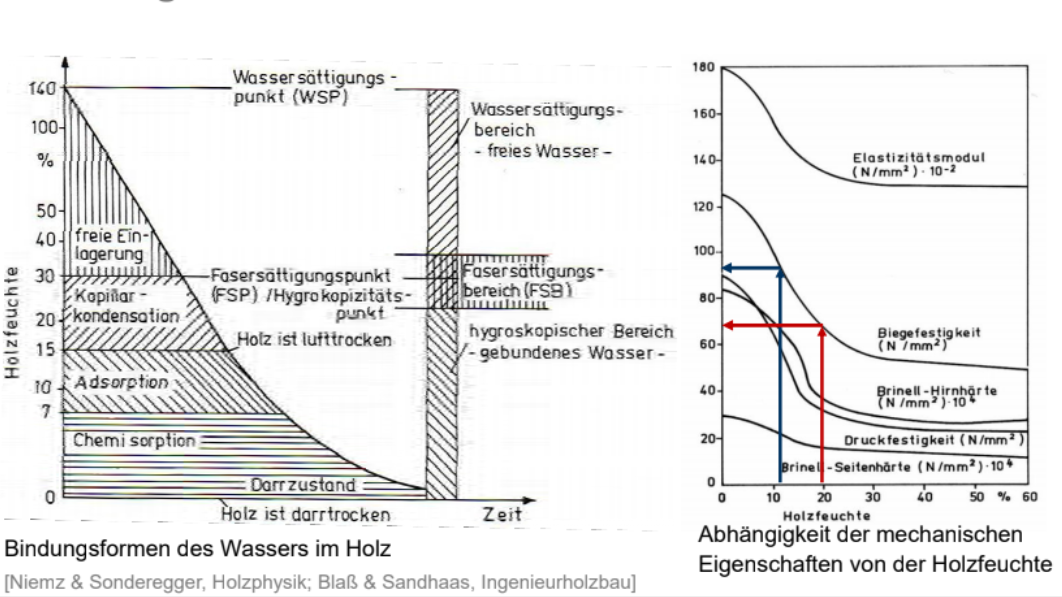
\includegraphics[width=0.45\textwidth]{Grafiken/Holzfeuchte/Wiederholung 01.png}
    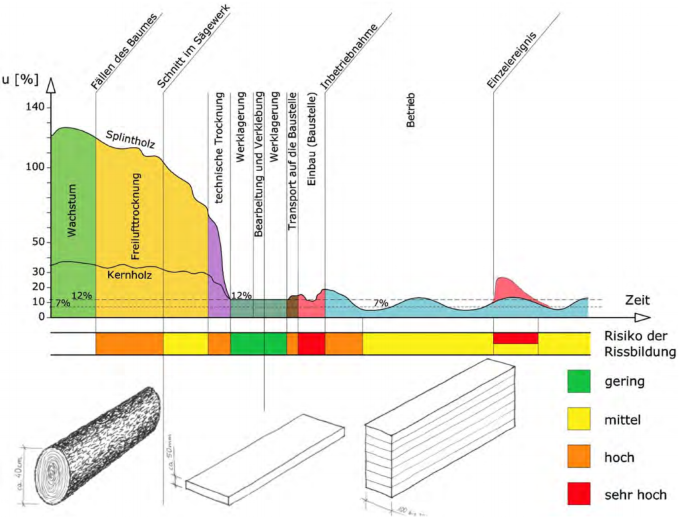
\includegraphics[width=0.45\textwidth]{Grafiken/Holzfeuchte/Wiederholung 02.png}\\

    \subsection{Problem-Anwendungsfelder}
        \begin{itemize}
            \item \textbf{Dachraum}
            \item \textbf{Lager}
            \item \textbf{Reiten}
            \item \textbf{Eislauf}
            \item \textbf{Brücke}
            \item Sport
            \item Versammlung
            \item Schwimmen
            \item Verkauf
            \item Produktion
        \end{itemize}

    \subsection{Häufigsten Schäden}
        \begin{itemize}
            \item Risse im Holz (4\%)
            \item Risse in Klebefugen (12\%)
            \item Risse in Holz und Klebefugen (30\%)
            \item Fäule (10\%)
            \item Schubbruch (5\%)
            \item Versagen der Verbindung (8\%)
            \item Stabilität (7\%)
        \end{itemize}

    \subsection{Häufigsten Ursachen}
        \begin{itemize}
            \item Niedrige/Hohe Holzfeuchte
            \item Holzfeuchtewechsel
            \item Querzugspannungen
            \item Qualität der Verklebung
            \item Biegespannungen
        \end{itemize}

    \subsection{Umgebungsbedingungen}
        Gebäudeklima Ergebnisse:
                \begin{itemize}
                    \item Schwimmhallen: konstantes und warmes Hallenklima\\
                        $\rightarrow$ konstante Holzfeuchte mit geringen Schwankungen und kleinen Gradienten \\
                        Ausnahme: Übergangsbereiche Innenbecken - Außenbecken
                    \item Sporthallen: konstantes, trockenes Klima\\
                        $\rightarrow$ geringe Holzfeuchten mit geringen Holzfeuchtegradienten;\\
                        $\rightarrow$ schonende Trocknung im ersten Winter nach Erstellung des Bauwerkes anstreben
                    \item Verkaufs- und Produktionshallen:\\
                        Verkaufshallen: vergleichbar mit Sporthallen;\\
                        Produktionshallen: unterschiedliche klimatische Bedingungen in Abhängigkeit der speziellen Nutzung\\
                        $\rightarrow$ Klimarandbedingungen objektspezifisch ermitteln
                    \item Reithallen: meist teiloffene, ungedämmte Bauweise\\
                        $\rightarrow$ großer Einfluss des Außenklimas; in Verbindung mit Sprinkleranlagen\\
                        $\rightarrow$ hohe Holzfeuchten mit merklichen Holzfeuchtegradienten, teilweise Tauwasserausfall
                    \item Landwirtschaftliche Hallen: vergleichbar mit Reithallen
                    \item Lagerhallen: zumeist offene Bauweise\\
                        $\rightarrow$ starker Einfluss des Außenklimas\\
                        $\rightarrow$ stark schwankende Holzfeuchten um MW von ca. $14 \%$
                    \item Eishallen: deutliche Klimaänderung zwischen Winter- und Sommermonaten (eisfreie Zeit)\\
                        $\rightarrow$ hohe Holzfeuchten mit starken jahreszeitlichen Schwankungen, größte Holzfeuchtegradiente nach Eisherstellung im Anschluss an Sommerpause, Einfluss durch Eisfläche
                    \item Zusammenfassung:
                        \begin{itemize}
                            \item Holzfeuchtegradienten in gedämmten und klimatisierten Bauwerken geringer als in Bauwerken mit stärkerem Einfluss des jahreszeitlich schwankenden Aussenklimas
                            \item Renovierungsarbeiten oder Nutzungsänderungen (temporär oder dauerhaft) können zu stark veränderten klimatischen Randbedingungen führen $\rightarrow$ schonende Änderung des Klimas anstreben (künstliche Luftbefeuchtung durch z.B. Verdunstungsbecken)
                            \item Einfluss von Lichtkuppeln $\rightarrow$ direkte Sonneneinstrahlung $\rightarrow$ höhere Temperaturen, geringere Luftfeuchte (Schutz durch z.B. Plattenwerkstoffe) 
                            \item Einfluss von Maschinen $\rightarrow$ höhere Temperaturen, geringere Luftfeuchte 
                            \item Feuchteeintrag durch z.B. Lagergüter (Pflanzen etc.) \item Filmbildende Anstriche haben deutlich dämpfende Wirkung auf Holzfeuchteänderungen und Größe der Holzfeuchtegradiente
                        \end{itemize}
                \end{itemize}

    \subsection{Effekte von Holzfeuchteänderungen}
        Trocknungsfolge - Risse
            \begin{itemize}
                \item Schwinden in tangentialer Richtung doppelt so stark wie in radialer Richtung
                \item Dies ruft Querzugspannungen im Querschnitt hervor
                \item Schwindrisse\\
                    $\rightarrow$ Schwindrisse um so größer, je größer der Querschnitt und je schneller die Trocknung
        \end{itemize}
        
        Trocknungsfolge - Krümmung und Verdrehung
            \begin{itemize}
                \item Schwinden in tangentialer Richtung doppelt so stark wie in radialer Richtung
                \item Krümmung und Verdrehung
                \item Über die Einschnittart lässt diese Gefahr verringern!
            \end{itemize}

        Feuchtewechsel - Relaxation
            \begin{itemize}
                \item Kriechen: Unter dem Kriechen versteht man den Verformungsanstieg im Zeitverlauf bei einer konstanten Spannung.
                \item (Relaxation: Die Relaxation hingegen beschreibt den Spannungsabfall im Zeitverlauf bei einer konstanten Dehnung.)
            \end{itemize}

        Rissbild und Spannungsbild bei freier Verformung\\
            \begin{minipage}{0.6\textwidth}
                \begin{itemize}
                    \item Querzugspannungen und Querdruckspannungen müssen im Gleichgewicht stehen! 
                    \item Nach Rissentstehung \\ $\rightarrow$ Querspannungen nur noch im Restquerschnitt
                \end{itemize}
            \end{minipage}
            \begin{minipage}{0.4\textwidth}
                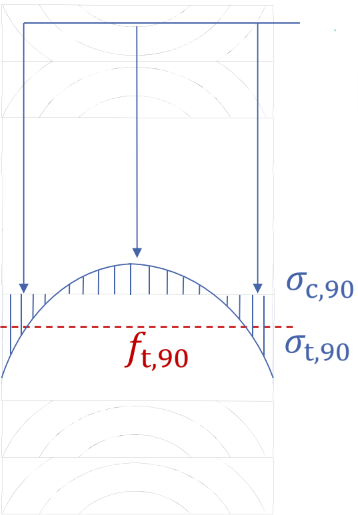
\includegraphics[width=0.4\textwidth]{Grafiken/Holzfeuchte/Risse Spannung 01.png}
                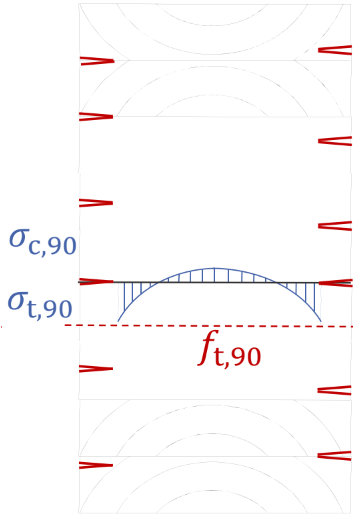
\includegraphics[width=0.4\textwidth]{Grafiken/Holzfeuchte/Risse Spannung 02.png}
            \end{minipage}

        Rissbild und Spannungsbild bei behinderter Verformung\\
            \begin{minipage}{0.6\textwidth}
                \begin{itemize}
                    \item z.B. Verbindungsmittelgruppe \\(Schlitzblech mit Stabdübeln)\\
                        $\rightarrow$ festes Auflager\\
                        $\rightarrow$ Querspannungen stehen
                        nicht mehr im Gleichgewicht\\
                        $\rightarrow$ größere und tiefere Risse
                \end{itemize}
            \end{minipage}
            \begin{minipage}{0.4\textwidth}
                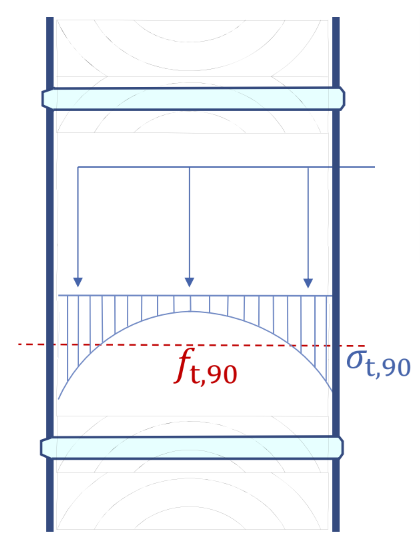
\includegraphics[width=0.4\textwidth]{Grafiken/Holzfeuchte/Risse behinderte Spannung 01.png}
                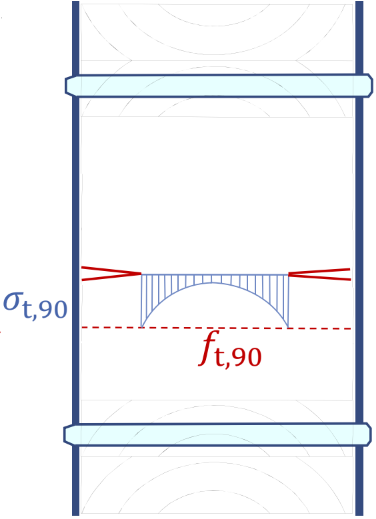
\includegraphics[width=0.35\textwidth]{Grafiken/Holzfeuchte/Risse behinderte Spannung 02.png}
            \end{minipage}
        Dübelkreis - Rissverteilung\\
                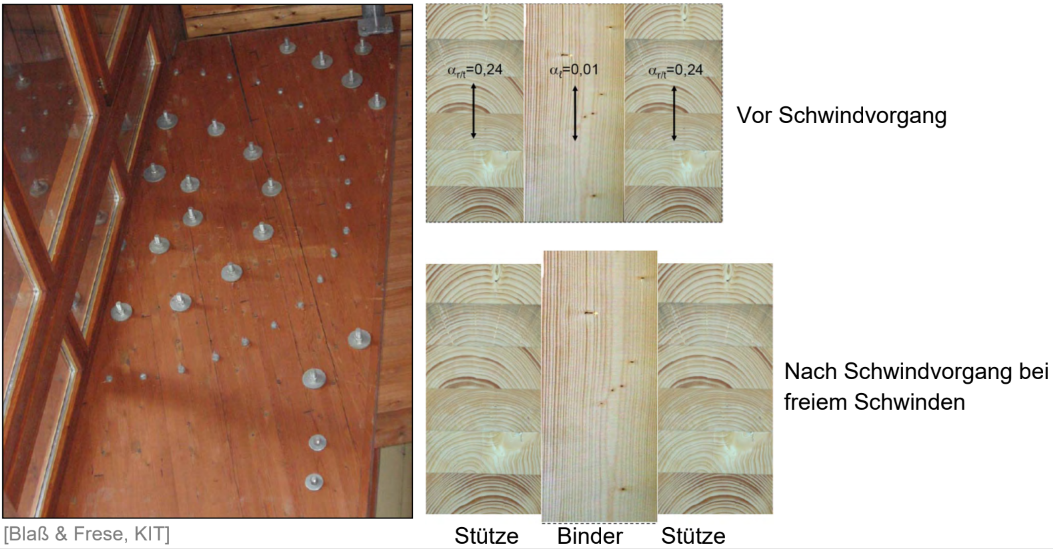
\includegraphics[width=0.45\textwidth]{Grafiken/Holzfeuchte/Duebelkreis Schwinden.png}


    \subsection{Verstärkte Bauteile unter Schwindbeanspruchung}



        Zusammenfassung:
            \begin{itemize}
                \item Freies Quellen/Schwinden durch Verstärkungselemente gesperrt
                \item Anordnung der Verstärkungselemente möglichst:
                    \begin{itemize}
                        \item in Querschnittsmitte unter Minimierung der Höhe der verstärkten Bereiche
                        \item in möglichst großen Abständen
                        \item Anordnung unter $45^{\circ}$ gutmütiger als $90^{\circ}$
                    \end{itemize}
                \item Unter $45^{\circ}$ angeordnete Verstärkungselemente führen zu höheren Tragähigkeiten von Trägern mit \\ Ausklinkungen und Durchbrüchen
                \item Die Einbaufeuchte sollte der späteren Ausgleichsfeuchte im Bauwerk entsprechen!
                \item Bei dauerhaft trockenem oder häufig wechselndem Klima
                    \begin{itemize}
                        \item Außen aufgeklebte Verstärkungselemente einsetzen\\
                        $\rightarrow$ Dämpfen den Prozess von Holzfeuchteänderungen oder Austrocknung.
                    \end{itemize}
                \item Der positive Verstärkungseffekt kann schon bei geringer Austrocknung $\left(1 \% \leq \Delta u \leq-2.5, \Delta u_{\text {mean }}=1.5 \%\right)$ durch die feuchteinduzierten Schwindspannungen neutralisiert werden.
            \end{itemize}

    
\newpage
\section{Erdbeben}

    \subsection{Historisches}
        \begin{itemize}
            \item Erster Entwurf/Erlass Bauvorschriften zu Erdbeben nach großem Erdbeben von 1755
            \item Holz und Holzverbindungen besonders vorteilhaft: $F=m\cdot a$ und Holz ist leicht
            \item Holzverbindungen weiterhin duktiles Verhalten (i.A.), kann somit Energie dissipieren 
            \\  $\rightarrow$ Holz jedoch als solches nicht!\\
                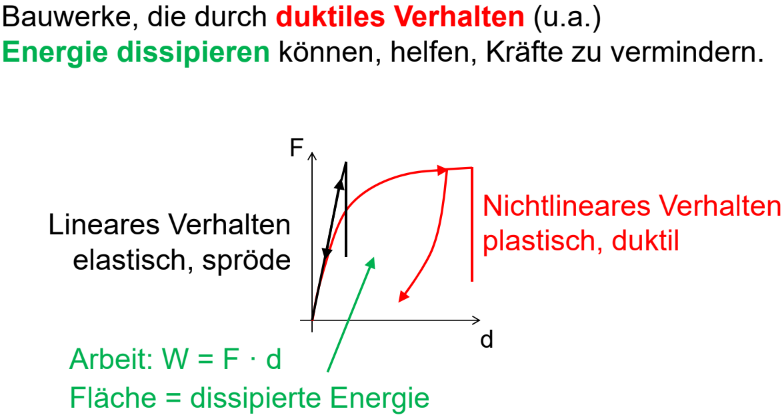
\includegraphics[width=0.45\textwidth]{Grafiken/Erdbeben/Dissipation-duktiles Verhalten.png}
            
        \end{itemize}

    \subsection{Interaktion Gebäude - Erdbeben}
        \begin{itemize}
            \item Nur Horizontalkräfte in dieser Vorlesung betrachtet
            \item Spitzenbodenbeschleunigung $a_g$ 
            \item (Lehrsches)Dämpfungsmaß: $\xi=\frac{d}{2\cdot m \cdot \omega}$ $\rightarrow$ 5\% als baupraktische Näherung\\
                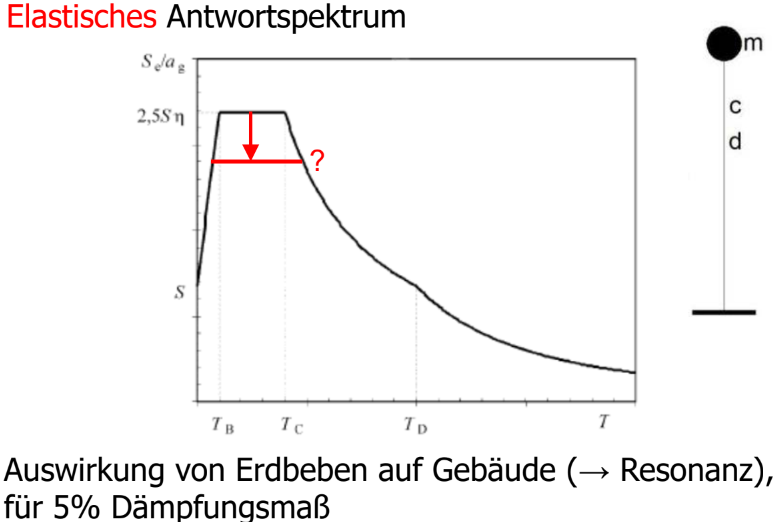
\includegraphics[width=0.45\textwidth]{Grafiken/Erdbeben/Elastisches Antwortspektrum.png}
            \item Eigenfrequenz: $f=f(m,c)$ [Hz]
            \item Eigenperiode: $T=T(m,c)$ [s]
            \item Eigenkreisfrequenz: $\omega = \sqrt{\frac{c}{m}}$ [Hz]
            \item $S_d = \frac{1}{\omega}\cdot S_v = \frac{1}{\omega^2}\cdot S_a$
                \begin{itemize}
                    \item $S_d$=Spektralverschiebung
                    \item $S_v$=Spektralgeschwindigkeit
                    \item $S_a$=Spektralbeschleunigung
                \end{itemize}
        \end{itemize}

        Abschließende Aussagen:
        \begin{itemize}
            \item Je duktiler das Verhalten, desto niedriger die im Gebäude auftretenden Kräfte
            \item ABER: Holz ist spröde (bei Biegung, Zug und Schub...)
            \item Holzverbindungen können jedoch duktil sein (falls sie gut entworfen sind!)
        \end{itemize}

        
    \subsection{Verbindungen - VCV VVDSt}
        \begin{itemize}
            \item Generelles Verhalten der Verbindungen:\\
                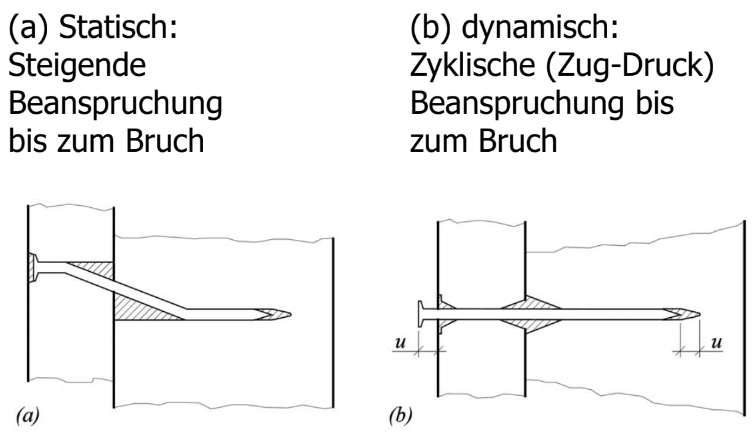
\includegraphics[width=0.45\textwidth]{Grafiken/Erdbeben/Verhalten Verbindungen.png}

            \item Statisch (monotoner) vs zyklisch (quasi-Statischer) Versuch:\\
                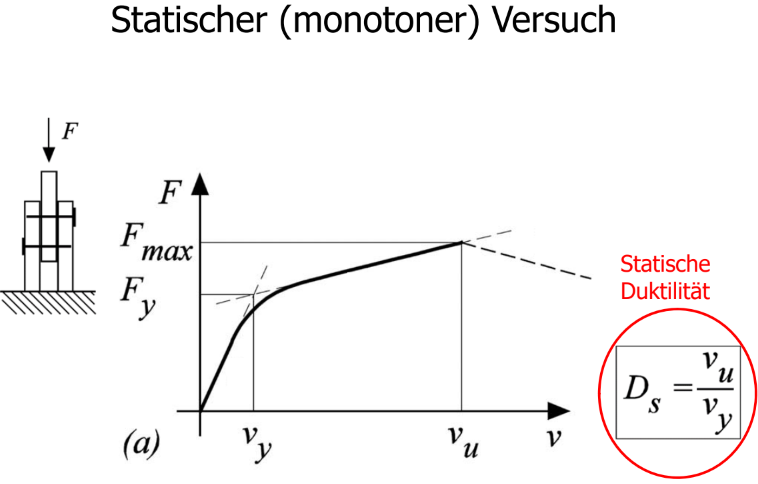
\includegraphics[width=0.45\textwidth]{Grafiken/Erdbeben/Statischer Versuch.png}
                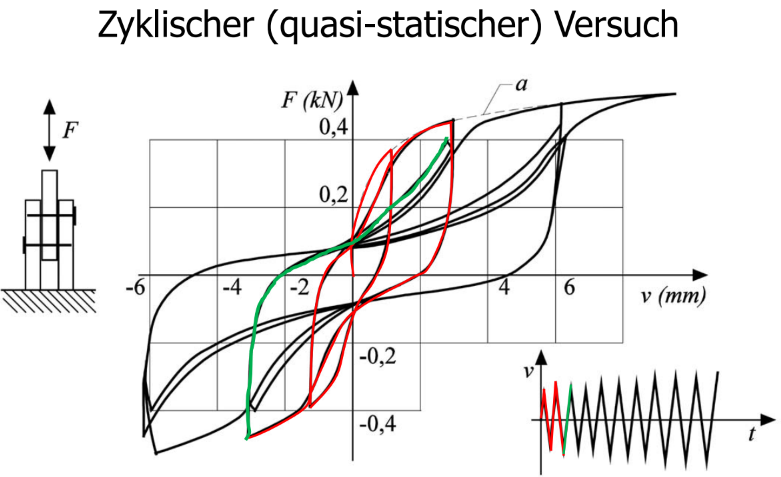
\includegraphics[width=0.45\textwidth]{Grafiken/Erdbeben/Zyklischer Versuch.png}

            \item Hysterese verschiedener Verbindungen:\\
                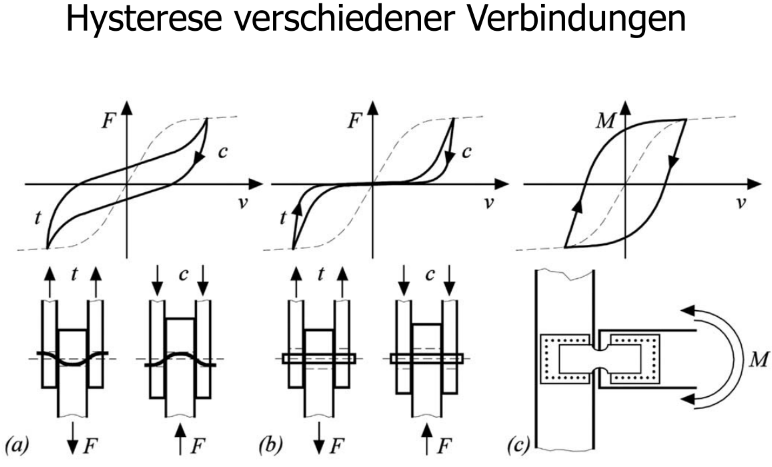
\includegraphics[width=0.45\textwidth]{Grafiken/Erdbeben/Hysterese versch. Verbindungen.png}
        \end{itemize}

    \subsection{Erdbebenbemessung}
        \begin{itemize}
            \item Rechtliches: Eurocode 8 (in Überarbeitung):
                \begin{itemize}
                    \item Bemessung von Neubauten, Altbauten, Ertüchtigungen
                    \begin{itemize}
                        \item Eurocode 8 basiert auf dem Konzept der Grenzzustände
                        \item Zwei Grenzzustände:
                        \item  \enquote{Tragfähigkeit} $\rightarrow$ kein Einsturz
                        \item  \sout{\text{\enquote{Gebrauchstauglichkeit}} $\rightarrow$ Schaden erlaubt} $\Rightarrow$ NA D
                    \end{itemize}
                \end{itemize}
            \item Berechnungsmethoden
                \begin{itemize}
                    \item Vereinfachtes Antwortspektrumverfahren (linear-elastisch)
                    \item Multimodales Antwortspektrumverfahren (linear-elastisch)
                    \item Nichtlineare statische (pushover) Berechnung
                    \item Nichtlineare Zeitverlaufsberechnung (dynamisch)
                \end{itemize}
                Genauigkeit und Komplexität nehmen zu

            \item Vereinfachtes Antwortspektrumverfahren
                \begin{itemize}
                    \item Darf bei Gebäuden angewendet werden,
                        \begin{itemize}
                            \item deren Antwort nicht wesentlich durch höhere Schwingungsformen beeinflusst wird.
                            \item die im Aufriss regelmäßig sind.
                        \end{itemize}
                        $\rightarrow$ Linear-elastische Bemessung nach Eurocode 5
                \end{itemize}

            \item Gesamterdbebenkraft $F_b$\\
                $F=m\cdot a$\\
                $F_b(T_1) = m \cdot a_g \cdot S \cdot \frac{2,5}{q} \cdot \eta$
                    \begin{itemize}
                        \item $T_1$ = Grundschwingungsdauer Bauwerk
                        \item $m$ = Gebäudemasse
                        \item $a_g$ = Bemessungswert der Spitzbodenbeschleunigung
                        \item $S$ = Bodenparameter
                        \item $\eta$ = Korrekturfaktor, siehe EC8 ($\eta$ für anderes Dämpfungsmaß)
                        \item q = Verhaltensbeiwert > 1 (berücksichtigt Energiedissipation)\\
                            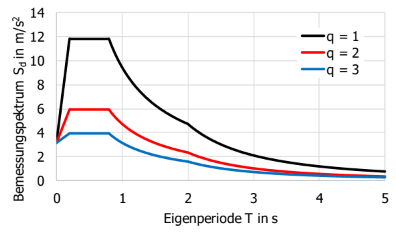
\includegraphics[width=0.45\textwidth]{Grafiken/Erdbeben/Verhaltensbeiwert.png}
                            
                    \end{itemize}

            \item Möglichkeiten der Bemessung:
                \begin{itemize}
                    \item Linear-elastisch, keine Energiedissipation
                        $\rightarrow$ \enquote{ q = 1 }
                    \item Abminderung von $F_b$ durch $\mathrm{q}>1$
                    \item Andere Lösungen zur Energiedissipation
                        $\rightarrow z$. B. base isolation
                \end{itemize}

            \item Duktilitätsklassen (DC) in EC8
                
                \resizebox{0.9\textwidth}{!}{%
                \begin{tabular}{|c|c|c|}
                \hline
                DCL (low) & $\gamma_M = 1,3$ & z.B.: Kragarme, Zwei- oder Dreigelenkbögen, Fachwerke mit Dübelverbindungen \\ \hline
                DCM (medium) & $\gamma_M = 1,0$ &  \\ \hline
                DCH (high) & $\gamma_M = 1,0$ & z.B.: Fachwerke mit Nagelverbindungen, Genagelte Wandscheiben mit genagelten Schubfeldern\\ \hline
                Overstrenght factor & $\gamma_M = 1,5$ & für spröde versagende Bauteile \\ \hline
                \end{tabular} } \vspace{1mm}

            \item Erdbebenkarte:\\
                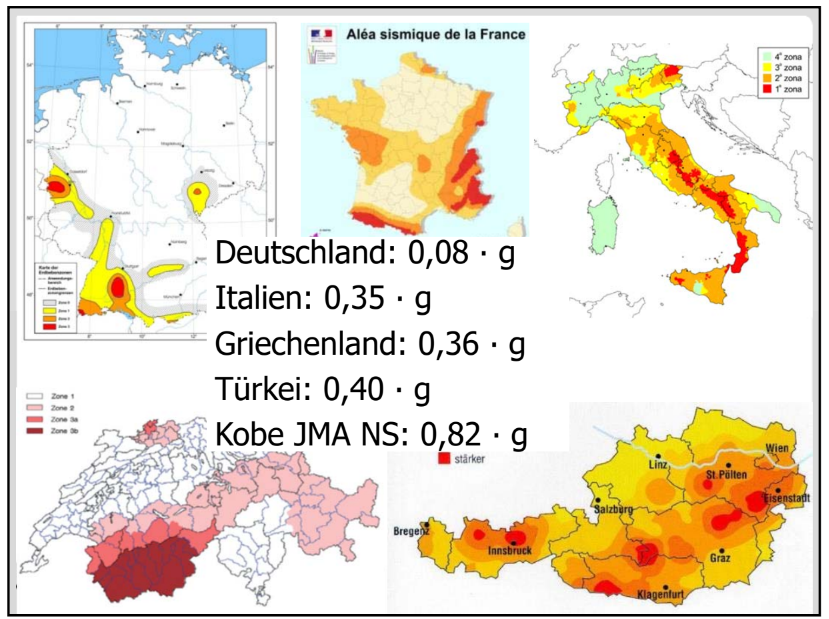
\includegraphics[width=0.55\textwidth]{Grafiken/Erdbeben/Erdbebenkarte.png}
                
        \end{itemize}


    \subsection{Qualitative Ziele}
        Grundlegende Prinzipien des Entwurfskonzepts:
            \begin{itemize}
                \item Konstruktive Einfachheit
                \item Regelmäßigkeit, Symmetrie und Redundanz
                \item Scheibenwirkung der Decken auf Geschossebene
            \end{itemize}

         \newpage   
        Ungünstig verbundene Bauteile:\\
                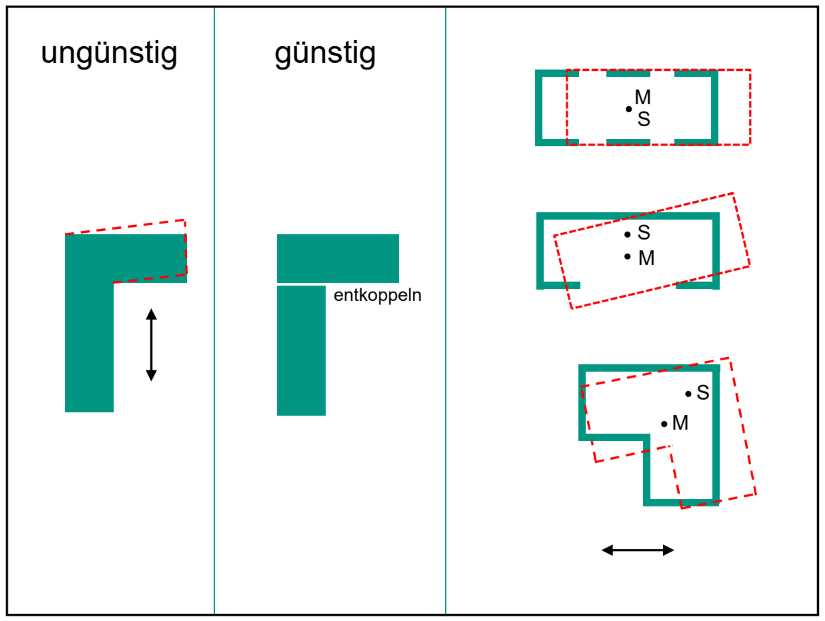
\includegraphics[width=0.45\textwidth]{Grafiken/Erdbeben/Unguenstig verbundene Bauteile.png}
            
    \subsection{Experimentelle Bestimmung von q}
            \begin{itemize}
                \item Bemessung Tragwerk nach Eurocode 8 für einen bestimmten q-Wert (e.g. q = 1) und gewähltes $\mathbf{a}_{\mathbf{g}, \mathbf{d}}$
                \item Teste das Tragwerk bis zum "near-collapse", indem $\mathbf{a}_{\mathbf{g}, \text {test}}$ erhöht wird
                \item Das Verhältnis von $\mathbf{a}_{\mathbf{g}, \text {test}}$ zu $\mathbf{a}_{\mathbf{g}, \mathbf{d}}$ ergibt den $\mathbf{q}$-Wert
            \end{itemize}


%\section{Klausurfragen}

 %   \begin{itemize}
  %      \item Wie werden Holztafeln miteinander verbunden?
  %  \end{itemize}
 
 
 
 
\end{document}